\documentclass{amsart}

\linespread{2}
% \usepackage{fontspec}
% \setmainfont{Open Dyslexic}


% PACKAGES ~~~~~~~~~~~~~~~~~~~~

\usepackage{amsfonts}
\usepackage{amssymb}  
\usepackage{amsthm} 
\usepackage{amsmath} 
\usepackage{caption}
\usepackage[inline]{enumitem}
\setlist{itemsep=0em, topsep=0em, parsep=0em}
\setlist[enumerate]{label=(\alph*)}
\usepackage{etoolbox}
\usepackage{stmaryrd} 
\usepackage[dvipsnames]{xcolor}
\definecolor{editcolour}{rgb}{0.7,0.1,0}
\definecolor{hrefcolour}{rgb}{0,0,0.7}

\usepackage[]{hyperref}
\hypersetup{colorlinks,linkcolor={hrefcolour},citecolor={hrefcolour},urlcolor={hrefcolour}}
\usepackage{graphicx}
\graphicspath{ {img/} }
\usepackage{mathtools}

\usepackage{tikz}
\usetikzlibrary{matrix,arrows,shapes,decorations.markings,decorations.pathreplacing}
\usepackage{todonotes}

% NEW COMMANDS ~~~~~~~~~~~~~~~~~~

% symbols
\renewcommand{\epsilon}{\varepsilon}
\newcommand{\op}{^{\scriptsize{ \textrm{op} } }}
\newcommand{\iso}{\cong}
\renewcommand{\equiv}{\simeq}

% categories
\newcommand{\A}{\cat{A}}
\newcommand{\B}{\cat{B}}
\newcommand{\C}{\cat{C}}
\newcommand{\D}{\cat{D}}
\newcommand{\E}{\cat{E}}
\renewcommand{\P}{\cat{P}}
\newcommand{\Q}{\cat{Q}}
\newcommand{\R}{\cat{R}}
\newcommand{\T}{\cat{T}}
\newcommand{\U}{\cat{U}}
\newcommand{\V}{\cat{V}}
\newcommand{\W}{\cat{W}}
\newcommand{\X}{\cat{X}}
\newcommand{\Y}{\cat{Y}}
\newcommand{\Z}{\cat{Z}}
\renewcommand{\AA}{\bicat{A}}
\newcommand{\BB}{\bicat{B}}
\newcommand{\CC}{\bicat{C}}
\newcommand{\DD}{\bicat{D}}
\newcommand{\EE}{\bicat{E}}
\newcommand{\PP}{\bicat{P}}
\newcommand{\QQ}{\bicat{Q}}
\newcommand{\RR}{\bicat{R}}
\newcommand{\TT}{\bicat{T}}
\newcommand{\UU}{\bicat{U}}
\newcommand{\VV}{\bicat{V}}
\newcommand{\WW}{\bicat{W}}
\newcommand{\XX}{\bicat{X}}
\newcommand{\YY}{\bicat{Y}}
\newcommand{\ZZ}{\bicat{Z}}
\newcommand{\AAA}{\dblcat{A}}
\newcommand{\BBB}{\dblcat{B}}
\newcommand{\CCC}{\dblcat{C}}
\newcommand{\DDD}{\dblcat{D}}
\newcommand{\EEE}{\dblcat{E}}
\newcommand{\MMM}{\dblecat{M}}
\newcommand{\PPP}{\dblcat{P}}
\newcommand{\QQQ}{\dblcat{Q}}
\newcommand{\RRR}{\dblcat{R}}
\newcommand{\SSS}{\dblcat{S}}
\newcommand{\TTT}{\dblcat{T}}
\newcommand{\UUU}{\dblcat{U}}
\newcommand{\VVV}{\dblcat{V}}
\newcommand{\WWW}{\dblcat{W}}
\newcommand{\XXX}{\dblcat{X}}
\newcommand{\YYY}{\dblcat{Y}}
\newcommand{\ZZZ}{\dblcat{Z}}

\newcommand{\Set}{\cat{Set}}
\newcommand{\Rel}{\cat{Rel}}
\newcommand{\Pos}{\cat{Pos}}
\newcommand{\Graph}{\cat{Graph}}
\newcommand{\RGraph}{\cat{RGraph}}
\newcommand{\Top}{\cat{Top}}
\newcommand{\Cat}{\cat{Cat}}
\newcommand{\Bicat}{\cat{Bicat}}
\newcommand{\DblCat}{\cat{DblCat}}
\newcommand{\Topos}{\cat{Topos}}
\newcommand{\Span}{\cat{Span}}
\newcommand{\Csp}{\cat{Cospan}}
\newcommand{\Gram}{\cat{Gram}}
\newcommand{\StrCsp}{\cat{StrCsp}}
\newcommand{\SSStrCsp}{\dblcat{S} \cat{trCsp}}
\newcommand{\StrCspGram}{\cat{StrCspGram}}
\newcommand{\MonSpCsp}{\dblcat{M} \cat{onSpCsp}}

% functors
\newcommand{\core}{\mathbf{core}}
\newcommand{\Lang}{\mathrm{Lang}}

% text formatting
\newcommand{\defn}[1]{\textbf{#1}}
\newcommand{\cat}[1]{\mathsf{#1}}
\newcommand{\bicat}[1]{\mathbf{#1}}
\newcommand{\dblcat}[1]{\mathbb{#1}}
\newcommand{\type}[1]{\mathtt{#1}}
\newcommand{\edit}[1]{\textcolor{editcolour}{(#1)}}

% arrows
\newcommand{\from}{\colon}
\newcommand{\rel}{\nrightarrow}
\newcommand{\To}{\Rightarrow}
\newcommand{\xto}[1]{\xrightarrow{#1}}
\newcommand{\monicto}{\rightarrowtail}
\newcommand{\dderiv}[2]{#1 \rightsquigarrow #2}
\newcommand{\deriv}[2]{#1 \rightsquigarrow^\ast #2}
\renewcommand{\gets}{\leftarrow}
\newcommand{\monicgets}{\leftarrowtail}
\newcommand{\xgets}[1]{\xleftarrow{#1}}
\newcommand{\spn}[3]{#2 \to #1 \times #3}
\newcommand{\tospan}{\xrightarrow{\mathit{sp}}}
\newcommand{\csp}[3]{#1 + #3 \to #2}
\newcommand{\tocospan}{\xrightarrow{\mathit{csp}}}

% OPERATORS ~~~~~~~~~~~~~~~~~~

\DeclareMathOperator{\Hom}{Hom}
\DeclareMathOperator{\id}{id}
\DeclareMathOperator{\im}{im}
\DeclareMathOperator{\Sub}{Sub}
\DeclareMathOperator{\colim}{colim}

% ENVIRONMENTS & COUNTERS ~~~~~~~~~~~

\newtheorem{theorem}{Theorem}[section]
\newtheorem{lemma}[theorem]{Lemma}
\newtheorem{proposition}[theorem]{Proposition}
\newtheorem{corollary}[theorem]{Corollary}

\theoremstyle{remark}
\newtheorem{remark}[theorem]{Remark}
\newtheorem{notation}[theorem]{Notation}

\theoremstyle{definition}
\newtheorem{example}[theorem]{Example} 
\newtheorem{definition}[theorem]{Definition}

\setcounter{tocdepth}{1} % Sets depth for table of contents. 

% TIKZ TYPES ~~~~~~~~~~~~~~~~~~~~~

% arrow head in middle of edge
\tikzset{->-/.style={decoration={%
      markings,
      mark=at position .5 with {\arrow{>}}},postaction={decorate}}
}

% arrow head user-positioned
\tikzset{->-pos/.style={decoration={%
      markings,
      mark=at position #1 with {\arrow{>}}},postaction={decorate}}
}

% arrow head in middle of edge
\tikzset{-|->/.style={decoration={%
      markings,
      mark=at position .5 with {\arrow{|}},mark=at position 1 with {\arrow{>}}},postaction={decorate}}
}

% INLINE DIAGRAMS ~~~~~~~~~~~~~~~

% walking reflexive graph
\newcommand{\rgraph}[2]{%
  \begin{tikzpicture}[scale=0.75,baseline=-3pt]
    \node (a) at (0,0) {$ #1 $};
    \node (b) at (1,0) {$ #2 $};
    \draw [->]
    ([yshift= 4pt]a.east) to ([yshift= 4pt]b.west);
    \draw [->]
    ([yshift=-4pt]a.east) to ([yshift=-4pt]b.west);
    \draw [->]
    (b.west) to (a.east);
  \end{tikzpicture}
}

% walking graph
\newcommand{\graph}[2]{%
  \begin{tikzpicture}[scale=0.75,baseline=-3pt]
    \node (a) at (0,0) {$ #1 $};
    \node (b) at (1,0) {$ #2 $};
    \draw [->]
    ([yshift=4pt]a.east) to ([yshift=4pt]b.west);
    \draw [->]
    ([yshift=-4pt]a.east) to ([yshift=-4pt]b.west);
  \end{tikzpicture}
}

% open tipped arrow
\newcommand{\opento}[2]{%
  \begin{tikzpicture}[scale=0.75,baseline=-3pt]
    \node (a) at (0,0) {$ #1 $};
    \node (b) at (1,0) {$ #2 $};
    \draw [->, open triangle 60]
    (a.east) to (b.west);
  \end{tikzpicture}
}

% inline horizontal arrow
\newlength\mylen
\settowidth\mylen{$\to$}

\newcommand{\horarrow}{%
  \to\kern-0.55\mylen\vline height 1.2ex depth
  -0.4pt\kern0.55\mylen}

% adjunction
\newcommand{\adjunction}[4]{%
  \begin{tikzpicture}[baseline=-3pt]
    \node (1) at (0,0) {\( #1 \)};
    \node (2) at (2,0) {\( #4 \)};
    \draw [->]
    ([yshift= 4pt]2.west) to
    node [above] {\scriptsize{ $ #2 $ }}
    ([yshift= 4pt]1.east);
    \draw [->]
    ([yshift= -4pt]1.east) to
    node [below] {\scriptsize{ $ #3 $ }}
    node [above,yshift= -1.5pt] {\scriptsize{$ \perp $}}
    ([yshift= -4pt]2.west);
  \end{tikzpicture}
  % 
}

\author{Daniel Cicala}
\title{Rewriting structured cospans}

% ~~~~~~~~~~~~~~~~~~~~~~~~~~~~~~~~~~~~~~~~
% 
% ~~~~~~~~~~~ begin document~~~~~~~~~~~~~~
% 
% ~~~~~~~~~~~~~~~~~~~~~~~~~~~~~~~~~~~~~~~~

\begin{document}
\maketitle{}

\begin{abstract}
  To foster the study of networks on an abstract level, we introduce
  the formalism of \emph{structured cospans}. A structured cospan is a
  diagram of the form $ La \to x \gets Lb $ built from a geometric
  morphism with left exact left adjoint
  $ L \dashv R \from \X \to \A $.  We show that this construction is
  functorial and results in a topos with structured cospans as objects.
  Additionally, structured cospans themselves are
  compositional. Combining these two perspectives, we define a double
  category of structured cospans.  We then leverage adhesive
  categories to create a theory of rewriting for structured cospans. A
  well-known result of graph rewriting is that a graph grammar induces
  the same rewrite relation as its underlying graph grammar. We
  generalize this result to topoi under the assumption that the
  subobject algebra on each context in the grammar is well-founded.
  This fact is used to provide a compositional framework for double
  pushout rewriting in a topos $ \X $ that is the domain of a
  geometric morphism.  
\end{abstract}

% ~~~~~~~~~~~~~~~~~~~~~~~~~~~~~~~~~~~~~~~~
% ~~~~~~~~~~~ introduction ~~~~~~~~~~~~~~~
% ~~~~~~~~~~~~~~~~~~~~~~~~~~~~~~~~~~~~~~~~

\section{Introduction}
\label{sec:Introduction}

% In such systems, local properties scale up to global
% properties.  This affords the ability to study local
% properties. Therefore, to be a reasonable syntax
%
% THE ABOVE SHOULD INFORM THE DIRECTION OF THE INTRO, NOT A HISTORY OF REWRITING

This paper fits into a program of codifying network theory into the
language of category theory
\cite{NetMods,PassiveNets,MrkvProc,RxNets,OpenPetri}. An important
aspect of this program falls within a theme common to many areas of
mathematics. That is the desire to study global properties using local
phenominon as illustrated by the advent of sheaf theory. A concept
related to the local study of systems is \emph{compositionality} which
occurs when properties of a system are completely determined by
properties of its sub-systems and the manner in which they are
connected together. A neccesary requirement of compositionality is the
existence of a mechanism by which to connect sub-systems together.  A
recent proposal for such a mechanism given by Baez and Courser
\cite{StrCsp} is called \emph{structured cospans}. 

The structured cospans serve as a syntax for systems. A
desirable feature of syntax is the ability to reflect a particular
sematics, specifically as it relates to distinct syntactical terms
with the same semantic representation.  One way to accomplish this is
using rewriting, which can be thought of as a relation similar to, but
more finely grained, than equality. The main goal of this paper is to
introduce a theory of rewriting for structured cospans.

To define a structured cospan, we begin with a functor
$ L \from \A \to \X $ where $ \A $ and $ \X $ have finite colimits and
$ \L $ preserves them. The objects of the category $ \X $ are your
systems of interest, for example graphs, Markov processes, Petri nets,
etc. The objects of $ \A $ are interfaces for the systems in $ \X
$. Often, this is $ \Set $.  Then $ L $ is the channel allowing the
interfaces to interact with the systems.  A more formal description
with that a structured cospan is a cospans of the form
$ La \to x \gets Lb $, where $ x $ is the system, $ La $ the inputs,
and $ Lb $ the outputs.  Another open system whose inputs are $ Lb $
can be connected to this via pushout, which is the familiar
composition in cospan categories
%
\[
  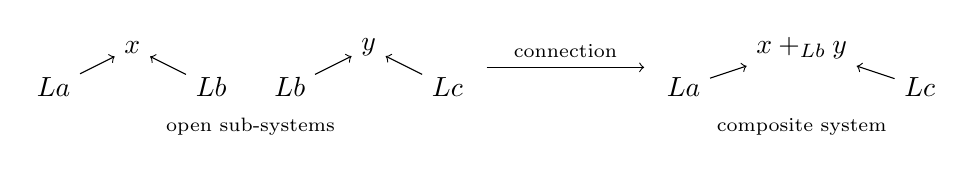
\begin{tikzpicture}
    \begin{scope}
      \node (1) at (0,0) {$ La $};
      \node (2) at (1,0.5) {$ x $};
      \node (3) at (2,0) {$ Lb $};
      \node (4) at (3,0) {$ Lb $};
      \node (5) at (4,0.5) {$ y $};
      \node (6) at (5,0) {$ Lc $};
      \draw [->] (1) to node [] {\scriptsize{$  $}} (2);
      \draw [->] (3) to node [] {\scriptsize{$  $}} (2);
      \draw [->] (4) to node [] {\scriptsize{$  $}} (5);
      \draw [->] (6) to node [] {\scriptsize{$  $}} (5);
      \node () at (2.5,-0.5) {\scriptsize{open sub-systems}};
    \end{scope}
    %
    \begin{scope}[shift={(8,0)}]
      \node (1) at (0,0) {$ La $};
      \node (2) at (1.5,0.5) {$ x +_{Lb} y $};
      \node (3) at (3,0) {$ Lc $};
      \draw [->] (1) to node [] {\scriptsize{$  $}} (2);
      \draw [->] (3) to node [] {\scriptsize{$  $}} (2);
      \node () at (1.5,-0.5) {\scriptsize{composite system}};
    \end{scope}
    %
    \draw [->] (5.5,0.25) to node [above] {\scriptsize{connection}} (7.5,0.25);    
  \end{tikzpicture}
\]
% 

In this program, \emph{functorial semantics} is used to describe
system behavior. That is, the semantics of such systems is captured by
a functor from our syntax category to a semantics category such as
$ \Set $, $ \Rel $, or $ \Pos $. The functoriality ensures composition
preserves properties of the system. There are early examples of applying
functorial semantics to possive linear networks \cite{PassiveNets},
Markov processes \cite{MrkvProc}, and chemical reaction networks \cite{ RxNets}.

In order to introduce rewriting into this structured cospan syntax, we
appeal to the most general class of objects that admit a rewriting
theory.  By this, we mean \emph{adhesive categories} whose axioms were
gathered specifically to encode the behavior of graph rewriting.
However, instead of working in the full generality of adhesive
categories, we restrict ourselves to elementary topoi, which are
examples of adhesive categories. To place ourseves into this context,
we define structured cospans stronger hypotheses than Baez and
Courser. Specifically, we begin with a geometric morphism, that is an
adjunction $ ( L \from \A \to \X ) \dashv ( R \from \X \to \A ) $
between topoi such that $ L $ preserves finite limits. In the systems
analogy, $ \A $, $ \X $, and $ L $ continue to serve as the
interfaces, systems, and interface channel. The compositional
structure remains and another perspective emerges where structured
cospans are objects with arrows between them.  The arrows are
commuting diagrams
%
\begin{equation} \label{eq:StrCsp-arrows}
\raisebox{-4.5ex}{
  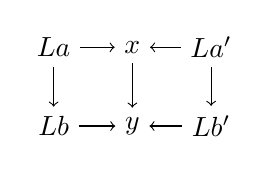
\begin{tikzpicture}
    \node (1t) at (0,1) {$ La $};
    \node (2t) at (1,1) {$ x $};
    \node (3t) at (2,1) {$ La' $};
    \node (1b) at (0,0) {$ Lb $};
    \node (2b) at (1,0) {$ y $};
    \node (3b) at (2,0) {$ Lb' $};
    \draw [->] (1t) to node [] {\scriptsize{$  $}} (2t);
    \draw [->] (3t) to node [] {\scriptsize{$  $}} (2t);
    \draw [->] (1b) to node [] {\scriptsize{$  $}} (2b);
    \draw [->] (3b) to node [] {\scriptsize{$  $}} (2b);
    \draw [->] (1t) to node [] {\scriptsize{$  $}} (1b);
    \draw [->] (2t) to node [] {\scriptsize{$  $}} (2b);
    \draw [->] (3t) to node [] {\scriptsize{$  $}} (3b);
  \end{tikzpicture}
}
\end{equation}
%
Structured cospans and their arrows form a category $ \StrCsp_L $ that
is the subject of our first result.

\begin{theorem*}[\ref{thm:strcsp-istopos}]
  $ \StrCsp_L $ is a topos.
\end{theorem*}

This theorem is neccesary to introduce a theory of rewriting to
structured cospans.

Thus far, we have referred to rewriting as if it is a single theory,
however there are actually several variants.  The relevant approach
for rewriting topoi uses \emph{double pushouts}.  Given a topos
$ \C $, we start with a finite set of spans in $ \C $
$ P \coloneqq \{ \ell_j \monicgets k_j \monicto r_j \} $ with monic
legs. These serve as \emph{rules} whose intution is that the object
$ \ell_j $ can be replaced by the object $ r_j $ while their common
subobject $ k_j $ is fixed.  This set of rules induces a set of
\emph{derived rules} $ P' $ comprised of any rules appearing on the
bottom row of a double pushout diagram of form
%
\[
  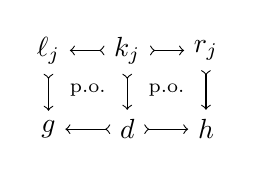
\begin{tikzpicture}
    \node (1) at (0,1) {$ \ell_j $};
    \node (2) at (1,1) {$ k_j $};
    \node (3) at (2,1) {$ r_j $};
    \node (4) at (0,0) {$ g $};
    \node (5) at (1,0) {$ d $};
    \node (6) at (2,0) {$ h $};
    \draw [>->] (2) to node [] {\scriptsize{$  $}} (1);
    \draw [>->] (2) to node [] {\scriptsize{$  $}} (3);
    \draw [>->] (5) to node [] {\scriptsize{$  $}} (4);
    \draw [>->] (5) to node [] {\scriptsize{$  $}} (6);
    \draw [>->] (1) to node [] {\scriptsize{$  $}} (4);
    \draw [>->] (2) to node [] {\scriptsize{$  $}} (5);
    \draw [>->] (3) to node [] {\scriptsize{$  $}} (6);
    \node () at (0.5,0.5) {\scriptsize{p.o.}};
    \node () at (1.5,0.5) {\scriptsize{p.o.}};
  \end{tikzpicture}
\]
%
whose top row belongs to $ P $. The object of study is the
\emph{rewrite relation} $ \deriv{g}{h} $ defined by, first, relating
objects if there is a rule in $ P' $ between them, then taking the
reflexive and transitive closure.

In this paper, we introduce a double pushout rewriting theory to
structured cospans. We start with some categorical bookkeeping with
the goal of encoding the rewrite relation functorially.  The first
categories we define are comprised of \emph{grammars}, a topos paired
with a finite set of rules, and a subcategory of the grammars of form
$ ( \StrCsp_L , P ) $ that run through geometric morphisms
$ ( L \from \A \to \X ) \dashv ( R \from \X \to \A ) $ and finite sets
of rules $ P $. There is a functor sending $ ( \StrCsp_L , P ) $ to
$ ( \StrCsp_L , P' ) $ where $ P' $ consists of rules derived from
$ P $.  We then apply another functor taking $ ( \StrCsp_L , P' ) $ to
the double category whose objects are from $ \A $, vertical arrows are
spans in $ \A $ with invertible legs, horizontal arrows are structured
cospans in $ \StrCsp_L $, and whose squares are generated by the rules
in $ P' $. The composite functor $ \Lang $ is called the language
functor. 

Using a double cateogry allows us to combine into a single structure
the connectability (horizontal composition) and rewritability
(vertical composition) of structured cospans.  The fact that this
actually is a double category \cite[Lem.~4.2]{CicCour_SpCspTopos}
ensures the compatibility of connecting and rewriting via the
interchange law. This compatability grants us the ability to decompose
a system into subsystems, rewrite those, then connect the
results.

What we are able to show is that rewriting the subsystems is
compatable with the rewrite relation.  To accomplish this, we turn to
Gadducci and Heckle \cite{Gadd_IndGraphTrans} who introduced an
inductive perspective for graph rewriting.  This is closely related to
our present goals so, while we work in a much more general context
than they, we follow the framework set in their paper.

When Ehrig, et. al.~, introdruced graph rewriting, they classified
the expressiveness of certain grammars.  One result that is relevant
here is that a set of rules $ \{ \ell_j \monicgets k_j \monicto
r_j \} $ has the same rewrite relation as the set of rules $ \{ \ell_j \monicgets k'_j \monicto
r_j \} $ where $ k'_j $ is the discrete graph underlying $ k_j $
\cite[Prop.~3.3]{Ehrig_GraphGram}.  Just as this fact was a keystone in
Gadducci and Heckle's work, we prove a modified version of it in
Theorem \cite{thm:production-same-rewrite-relation-as-discrete}. To
understand the following statement, we use the notation $ P_\flat $ to
refer to the set of rules obtained from $ P = \{ \ell_j \monicgets k_j
\monicto r_j \} $ by restricting the the span lets along the counit $
LRk_j \to k_j $ of the comonad $ LR $.

\begin{theorem*}
Fix a geometric morphism $ L \dashv R \from \X \to \A $ with monic
counit. Let $ ( \X , P ) $ be a grammar such that for every
$ \X $-object $ x $ in the apex of a production of $ P $, the Heyting
algebra $ \Sub (x) $ is well-founded.  The rewriting relation for a
grammar $ ( \X , P ) $ is equal to rewriting relation for the grammar
$ ( \X , P_{\flat} ) $
\end{theorem*}

To attach this result to our goal of lifting the rewriting of subsystems to
rewriting systems, recall that in the analogy between structured cospans
and systems, the topos $ \X $ is where the systems live.  That is, our
objective is to study the rewriting relation induced by the grammar $
( \X , P ) $ locally.  This theorem states that we can instead study
the rewriting relation for the grammar $ ( \X , P_\flat ) $ because it
is the same.  It is the bridge to encoding the rewrite relation for
$ ( \X , P ) $ in its language.   

In order to study $ ( \X,P ) $ locally, we need to break it into
pieces.  This is where structured cospans come into the story.  











\ref{sec:StrCsp}\todo{finish the story}


The structure of the paper is as follows.  Section \ref{sec:StrCsp}
defines structured cospans, the main object of study. There are two
perspectives on structured cospans and we realize this by building two
separate categories.  The first category $ \StrCsp_L $, mentioned
above, has structured cospans as objects and commuting diagrams
\eqref{eq:StrCsp-arrows} as arrows. The first result, and the keystone
of the paper, is that $ \StrCsp_L $ is a topos.  This grants us access
to the theory of adhesive rewriting.  The second category, and the one
introduced by Baez and Courser \cite{StrCsp} views structured cospans
as arrows.  We then combine these two perspectives into a double
category.

In Section \ref{sec:inductive-rewriting-structured-cospans}, we sweep
over the basics of graph rewriting and cover the inductive viewpoint.
We also recall the theory of adhesive categories before applying it to
structured cospans in a categorical framework. We start with
\emph{grammars}. There are two types of grammars we are interested in.
The first involves pairing an adhesive category $ \C $ with a set of
productions $ P $ inside $ \C $. These form a category.  There is a
subcategory we use too, consisting of grammars $ ( \StrCsp_L , P ) $
where $ P $ is a set of spans in $ \StrCsp_L $ of the form
%
\[
  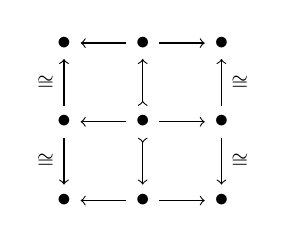
\begin{tikzpicture}
    \node (1t) at (0,2) {$ \bullet $};
    \node (2t) at (1,2) {$ \bullet $};
    \node (3t) at (2,2) {$ \bullet $};
    \node (1m) at (0,1) {$ \bullet $};
    \node (2m) at (1,1) {$ \bullet $};
    \node (3m) at (2,1) {$ \bullet $};
    \node (1b) at (0,0) {$ \bullet $};
    \node (2b) at (1,0) {$ \bullet $};
    \node (3b) at (2,0) {$ \bullet $};
    \draw [->] (2t) to node [] {\scriptsize{$  $}} (1t);
    \draw [->] (2t) to node [] {\scriptsize{$  $}} (3t);
    \draw [->] (2m) to node [] {\scriptsize{$  $}} (1m);
    \draw [->] (2m) to node [] {\scriptsize{$  $}} (3m);
    \draw [->] (2b) to node [] {\scriptsize{$  $}} (1b);
    \draw [->] (2b) to node [] {\scriptsize{$  $}} (3b);
    \draw [->] (1m) to node [left] {\scriptsize{$ \iso $}} (1t);
    \draw [->] (1m) to node [left] {\scriptsize{$ \iso $}} (1b);
    \draw [>->] (2m) to node [] {\scriptsize{$  $}} (2t);
    \draw [>->] (2m) to node [] {\scriptsize{$  $}} (2b);
    \draw [->] (3m) to node [right] {\scriptsize{$ \iso $}} (3t);
    \draw [->] (3m) to node [right] {\scriptsize{$ \iso $}} (3b);
  \end{tikzpicture}
\]
% 
and fitting them into a category $ \StrCspGram $.  Given a grammar
$ ( \C , P ) $, we define the rewriting relation on the objects
of $ \C $ using double pushouts in a manner similar to that as
was done for graphs.  However, we provide a functorial characterization
as well. Namely, the functor $ D \from \Gram \to \Gram $
that send a grammar $ ( \C , P ) $ to the grammar $ ( \C
, P') $ where a production $ g \gets d \to h $ belongs to $ P' $ if
there is a double pushout diagram
%
\[
  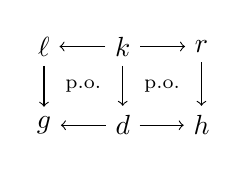
\begin{tikzpicture}
    \node (1t) at (0,1) {$ \ell $};
    \node (2t) at (1,1) {$ k $};
    \node (3t) at (2,1) {$ r $};
    \node (1b) at (0,0) {$ g $};
    \node (2b) at (1,0) {$ d $};
    \node (3b) at (2,0) {$ h $};
    \draw [->] (2t) to node [] {\scriptsize{$  $}} (1t);
    \draw [->] (2t) to node [] {\scriptsize{$  $}} (3t);
    \draw [->] (2b) to node [] {\scriptsize{$  $}} (1b);
    \draw [->] (2b) to node [] {\scriptsize{$  $}} (3b);
    \draw [->] (1t) to node [] {\scriptsize{$  $}} (1b);
    \draw [->] (2t) to node [] {\scriptsize{$  $}} (2b);
    \draw [->] (3t) to node [] {\scriptsize{$  $}} (3b);
    \node () at (0.5,0.5) {\scriptsize{p.o.}};
    \node () at (1.5,0.5) {\scriptsize{p.o.}};
  \end{tikzpicture}
\]
% 
such that the top row is a production in $ P $. We then define a
semantics functor $ S \from \Gram \to \DblCat $ valued in double
categories.  These semantics capture the compositionality of the
structured cospans and also the rewriting.  The \emph{language} of a
grammar is its image under the composite functor $ SD $. Our main
result is Theorem \ref{thm:inductive-rewriting}. Given a grammar
$ ( \X , P ) $ on a topos $ \X $ fitting into a suitable geometric
morphism $ L \dashv R \from \X \to \A $, then we construct a grammar $
( \StrCsp_L , Q ) $ such that $ g $ is related to $ h $ from the
rewriting relation on the grammar $ ( \X , P ) $ exactly when there is
a square in the double category $ SD ( \StrCsp_L , Q ) $ of the form
\[
    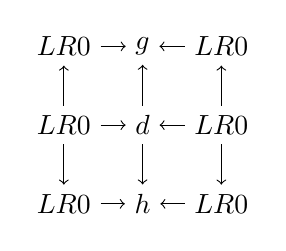
\begin{tikzpicture}
      \node (1t) at (0,2) {$ LR 0 $};
      \node (2t) at (1,2) {$ g $};
      \node (3t) at (2,2) {$ LR 0 $};
      \node (1m) at (0,1) {$ LR 0 $};
      \node (2m) at (1,1) {$ d $};
      \node (3m) at (2,1) {$ LR 0 $};
      \node (1b) at (0,0) {$ LR 0 $};
      \node (2b) at (1,0) {$ h $};
      \node (3b) at (2,0) {$ LR 0 $};
      \draw [->] (1t) to node [] {\scriptsize{$  $}} (2t);
      \draw [->] (3t) to node [] {\scriptsize{$  $}} (2t);
      \draw [->] (1m) to node [] {\scriptsize{$  $}} (2m);
      \draw [->] (3m) to node [] {\scriptsize{$  $}} (2m);
      \draw [->] (1b) to node [] {\scriptsize{$  $}} (2b);
      \draw [->] (3b) to node [] {\scriptsize{$  $}} (2b);
      \draw [->] (1m) to node [] {\scriptsize{$  $}} (1t);
      \draw [->] (1m) to node [] {\scriptsize{$  $}} (1b);
      \draw [->] (2m) to node [] {\scriptsize{$  $}} (2t);
      \draw [->] (2m) to node [] {\scriptsize{$  $}} (2b);
      \draw [->] (3m) to node [] {\scriptsize{$  $}} (3t);
      \draw [->] (3m) to node [] {\scriptsize{$  $}} (3b);
    \end{tikzpicture}
\]
Simply stated, if $ \X $ contains a type of network, then the
rewritings on networks of type $ \X $ can be understood by rewriting
on pieces of the network inside of $ ( \StrCsp , Q ) $ then gluing
them back together.

The author would like to thank John Baez and Fabio Gadducci for
helpful conversations.

% ~~~~~~~~~~~~~~~~~~~~~~~~~~~~~~~~~~~~~~~~
% ~~~~~~~~~~~ structured cospans~~~~~~~~~~
% ~~~~~~~~~~~~~~~~~~~~~~~~~~~~~~~~~~~~~~~~

\section{Structured Cospans}
\label{sec:StrCsp}

Structured cospans were introduced by Baez and Courser \cite{StrCsp}
to provide syntax for compositional systems.  Their work has two aims:
maximize the generality of the structured cospan construction using
double categories and also to compare structured cospans to Fong's
decorated cospans \cite{DecorCsp}, an alternative syntax. Because
structured cospans are a syntax, we want to set up a framework that
can reflect the semantics. This paper proposes such a framework, for
which we use the notion of double pushout rewriting. Due to our
motivation, we assume different (but not disjoint) hypothesis than
Baez and Courser.  The purpose of this section is to set our
hypothesis and explore the nature of structured cospans in this
context. Instead of embarking on a mission to fully lay out a theory
of structured cospans, we restrain ourselves to just those aspects
needed to introduce rewriting.  

To be specific, in this section we make explicit competing
perspectives.  The first is looking at structured cospans as objects
of a category with appropriate morphisms between them. The second
takes structured cospans as morphisms between certain ``interfaces''.
The latter perspective encode the compositional structure. We then
complete this section by marrying the two perspectives using double categories.

Fix an arbitrary geometric morphism $ L \dashv R \from \X \to \A
$. This is an adjunction
%
\[
  \adjunction{\X}{L}{R}{\A}
\]
%
between (elementary) topoi with $ L $ left exact. Because spans and
cospans factor heavily into this work, we use the notation
%
\(
 (f,g) \from \spn{x}{y}{z}
\)
% 
for a span
%
\[
  x \xgets{f} y \xto{g} z
\]
%
and
%
\(
  (f,g) \from \csp{x}{y}{z}
\)
% 
for a cospan
%
\[
  x \xto{f} y \xgets{g} z.
\]
% 
Because all of the categories in this paper have products and
coproducts, this notation is sensible.

% ~~~~~~~~~~~~~~~~~~~~~~~~
% ~~~~~~~~~~~~~~~~~~~~~~~~

\subsection{Structured cospans as objects}
\label{sec:StrCspAsObject}

\begin{definition}\label{df:strcsp}
  A \defn{structured cospan} is a cospan of the form
  $ \csp{La}{x}{Lb} $.  When we want to emphasize $ L $, we use the
  term $ L $-structured cospans.
\end{definition}

The motivating force behind inventing structured cospans is to
describe open systems, and so we do not hesitate to draw on the the
intuition of open systems to better understand structured cospans.
For instance, one should view the topos $ \X $ as consisting of closed
systems and their morphisms. By a \emph{closed system}, we mean a
system that cannot interact with the outside world. The topos $ \A $
should be thought to contain possible interfaces for the closed
systems. Equipping a closed system with an interface provides the
system a way to interact with compatible elements of the outside
world. Such a system is no longer closed, and so we call it an
\emph{open system}. The left adjoint $ L $ sends these interfaces into
$ \X $ so that they might interact with the closed systems. The right
adjoint $ R $ can be though of as returning all possible interface
elements of a closed system.

Through this perspective, a structured cospan consists of a closed
system $ x $ equipped with the interface described by the arrows from
$ La $ and $ Lb $. By ignoring questions of causality, we may safely
consider $ La $ as the input to $ x $ and $ Lb $ as the output.  As
expected, a morphism of open system ought to respect these components.

\begin{definition} \label{df:morph-of-strcsp}

  A morphism from one $ L $-structured cospan
  %
  \(
    \csp{La}{x}{Lb}
  \)
  %
  to another
  %
  \(
    \csp{Lc}{y}{Ld}
  \)
  % 
  is a triple of arrows $ ( f,g,h ) $ that fit into the commuting
  diagram
  \[
    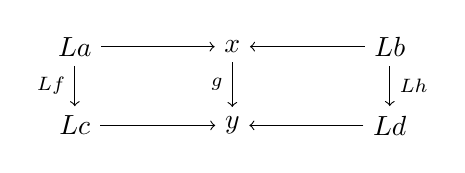
\begin{tikzpicture}
      \node (1) at (-2,1) {\( La \)};
      \node (2) at (0,1) {\( x \)};
      \node (3) at (2,1) {\( Lb \)};
      \node (4) at (-2,0) {\( Lc \)};
      \node (5) at (0,0) {\( y \)};
      \node (6) at (2,0) {\( Ld \)};
      \draw [->] (1) to node [above] {\scriptsize{\(  \)}} (2);
      \draw [->] (3) to node [above] {\scriptsize{\(  \)}} (2);
      \draw [->] (4) to node [below] {\scriptsize{\(  \)}} (5);
      \draw [->] (6) to node [below] {\scriptsize{\(  \)}} (5);
      \draw [->] (1) to node [left] {\scriptsize{\( Lf \)}} (4);
      \draw [->] (2) to node [left] {\scriptsize{\( g \)}} (5);
      \draw [->] (3) to node [right] {\scriptsize{\( Lh \)}} (6);
    \end{tikzpicture}
  \]
\end{definition}

It is easy to check that $ L $-structured cospans and their morphisms
form a category, which we denote by $ \StrCsp_L $.

\begin{example}[Open graphs] \label{ex:open-graphs}

  Systems theory is intimately tied with graph theory.  A natural
  example of a structured cospan is an \emph{open graph}. While this
  notion is not new \cite{DixKiss_OpenGraphs,Gadd_IndGraphTrans}, our
  infrastructure generalizes it.

  Denote by $ \RGraph $ the category of (directed reflexive
  multi-) graphs. There is an adjunction
  %
  \[
    \adjunction{\RGraph}{L}{R}{\Set}
  \]
  % 
  where $ Rx $ is the node set of graph $ x $ and $ La $ is the
  edgeless graph with node set $ a $. An \defn{open graph} is a cospan
  %
  \(
      \csp{La}{x}{Lb}
  \)
  % 
  for sets $ a $, $ b $, and graph $ x $. An illustrated example, with
  the reflexive loops suppressed, is
  %
  \[
    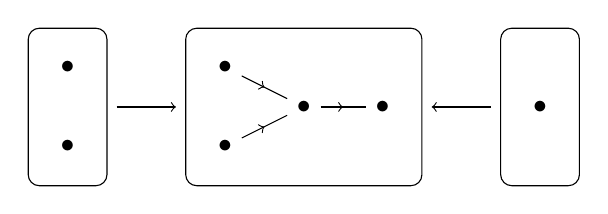
\begin{tikzpicture}
      %
      \begin{scope} % left graph
      \node (1) at (0,1) { \( \bullet \) };
      \node (2) at (0,0) { \( \bullet \) };
      \draw [rounded corners] (-0.5,-0.5) rectangle (0.5,1.5);
      \end{scope}
      %
      \begin{scope}[shift={(2,0)}] % center graph
      \node (1) at (0,1) {\( \bullet \)};
      \node (2) at (0,0) {\( \bullet \)};
      \node (3) at (1,0.5) {\( \bullet  \)};
      \node (4) at (2,0.5) {\( \bullet  \)};
      \draw [->-] (1) to (3);
      \draw [->-] (2) to (3);
      \draw [->-] (3) to (4);
      \draw [rounded corners] (-0.5,-0.5) rectangle (2.5,1.5);
      \end{scope}
      %
      \begin{scope}[shift={(6,0)}] % right graph
      \node (1) at (0,0.5) {\( \bullet \)};
      \draw [rounded corners] (-0.5,-0.5) rectangle (0.5,1.5);
      \end{scope}
      %
      \begin{scope} % graph morphisms
        \node (1) at (0.5,0.5) {};
        \node (2) at (1.5,0.5) {};
        \node (3) at (4.5,0.5) {};
        \node (4) at (5.5,0.5) {};
        \draw [->] (1) to (2);
        \draw [->] (4) to (3);
      \end{scope}
    \end{tikzpicture}
  \]
  % 
  The boxed items are graphs and the arrows between boxes are graph
  morphisms defined as suggested by the illustration.  In total, the
  three graphs and two graph morphisms make up a single open graph
  whose inputs and outputs are, respectively, the left and right-most
  graphs.
    
\end{example}

% what good is the open bit?

Having seen this example, it becomes more apparent about how open
systems can ``connect'' together. Given another open graph whose
inputs coincide with the outputs of the graph above, we can connect
the inputs and outputs together to create a new open graph. By passing
from graphs to open graphs, we are introducing
\emph{compositionality}. The category $ \StrCsp_{L} $ does not encode
the compositional structure, but we introduce a new category
$ \Csp_L $ in Section \ref{sec:StrCsp-as-Arrows} which does.

We now come to the first of our main results: that $ \StrCsp_L $ is a
topos. In terms of this paper, this result is critical because it
allows for the introduction of rewriting onto structured cospans.

\begin{theorem}
\label{thm:strcsp-istopos}
  The category $ \StrCsp_L $ is a topos.
\end{theorem}

\begin{proof}
  The category $ \StrCsp_L $ constructed using the geometric morphism
  $ L \dashv R \from \X \to \A $ is equivalent to the category
  whose objects are cospans of form
  %
  \(
    \csp{a}{Rx}{b}
  \)
  % 
  and morphisms are triples $ ( f,g,h ) $ fitting into the commuting
  diagram
  %
  \[
    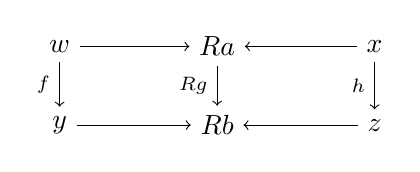
\begin{tikzpicture}
      \node (1) at (-2,1) {\( w \)};
      \node (2) at (0,1) {\( Ra \)};
      \node (3) at (2,1) {\( x \)};
      \node (4) at (-2,0) {\( y \)};
      \node (5) at (0,0) {\( Rb \)};
      \node (6) at (2,0) {\( z \)};
      \draw [->] (1) to  node [] {\scriptsize{\(  \)}} (2);
      \draw [->] (3) to node [] {\scriptsize{\(  \)}} (2);
      \draw [->] (4) to node [] {\scriptsize{\(  \)}} (5);
      \draw [->] (6) to node [] {\scriptsize{\(  \)}} (5);
      \draw [->] (1) to node [left] {\scriptsize{\( f \)}} (4);
      \draw [->] (2) to node [left] {\scriptsize{\( Rg \)}} (5);
      \draw [->] (3) to node [left] {\scriptsize{\( h \)}} (6); 
    \end{tikzpicture}
  \]
  % 
  This, in turn, is equivalent to the comma category
  $ ( \A \times \A \downarrow \Delta R ) $, where
  $ \Delta \from \A \to \A \times \A $ is the diagonal functor. But
  the diagonal functor is right adjoint to taking binary
  coproducts. That means $ \Delta R $ is also a right adjoint and,
  furthermore, that $ ( \A \times \A \downarrow \Delta R ) $ is an
  instance of Artin gluing \cite{Wraith_ArtinGlue}, hence a topos.
\end{proof}

We now show that the construction of $ \StrCsp_L $ is actually functorial.

\begin{theorem} \label{thm:strcsp-isfunctorial}

  There is a functor
  %
  \[
    \StrCsp_{(-)} \from
    [ \bullet \to \bullet , \Topos ]
    \to
    \Topos
  \]
  % 
  defined by  
  \[
    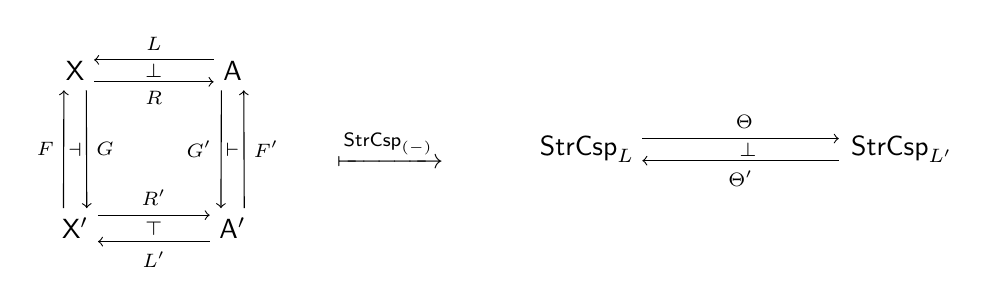
\begin{tikzpicture}
      \begin{scope}
      \node (1) at (-1,1) {\( \X \)};
      \node (2) at (-1,-1) {\( \X' \)};
      \node (3) at (1,1) {\( \A \)};
      \node (4) at (1,-1) {\( \A' \)};
      \draw [->] (1.-60) to node [right] {\scriptsize{\( G \)}} (2.60);
      \draw [<-] (1.-120) to node [left] {\scriptsize{\( F \)}} (2.120);
      \draw [<-] (1.30) to node [above] {\scriptsize{\( L \)}} (3.150);  
      \draw [->] (1.-30) to node [below] {\scriptsize{\( R \)}} (3.-150);
      \draw [->] (2.30) to node [above] {\scriptsize{\( R' \)}} (4.150);
      \draw [<-] (2.-30) to node [below] {\scriptsize{\( L' \)}} (4.-150);      
      \draw [<-] (3.-60) to node [right] {\scriptsize{\( F' \)}} (4.60);
      \draw [->] (3.-120) to node [left] {\scriptsize{\( G' \)}}
      (4.120);
      \node (5) at (0,-1) {\scriptsize{\( \top \)}};
      \node (6) at (0,1) {\scriptsize{\( \perp \)}};
      \node (7) at (-1,0) {\scriptsize{\( \dashv \)}};
      \node (8) at (1,0) {\scriptsize{\( \vdash \)}};
      \end{scope}
     % 
      \begin{scope}[shift={(3,0)}]
      \node (1) at (0,0) { $\xmapsto{ \StrCsp_{(-)} }$ };
      \end{scope}
      %
      \begin{scope}[shift={(5.5,0)}]
      \node (1) [inner sep=0.1cm] at (0,0) {\( \StrCsp_{L} \)};
      \node (2) [inner sep=0.15cm] at (4,0) {\( \StrCsp_{L'} \)};
      \node (3) at (2,0) {\scriptsize{ \( \perp \) }};
      \draw [->]
        ([yshift= 4pt]1.east) to
        node [above] {\scriptsize{ \( \Theta \) }}
        ([yshift= 4pt]2.west);
      \draw [->]
        ([yshift= -4pt]2.west) to
        node [below] {\scriptsize{ \( \Theta' \) } }
        ([yshift= -4pt]1.east);  
      \end{scope}
    \end{tikzpicture}
  \]
  % 
  which is in turn given by
  %
  \[
    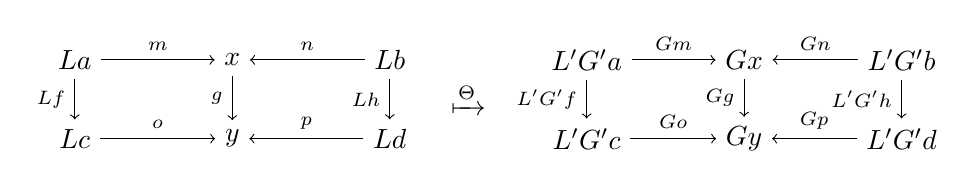
\begin{tikzpicture}
      \begin{scope}
      \node (1) at (-2,1) {\( La \)};
      \node (2) at (0,1) {\( x \)};
      \node (3) at (2,1) {\( Lb \)};
      \node (4) at (-2,0) {\( Lc \)};
      \node (5) at (0,0) {\( y \)};
      \node (6) at (2,0) {\( Ld \)};
      \draw [->] (1) to node [above] {\scriptsize{\( m \)}} (2);
      \draw [->] (3) to node [above] {\scriptsize{\( n \)}} (2);
      \draw [->] (4) to node [above] {\scriptsize{\( o \)}} (5);
      \draw [->] (6) to node [above] {\scriptsize{\( p \)}} (5);
      \draw [->] (1) to node [left] {\scriptsize{\( Lf \)}} (4);
      \draw [->] (2) to node [left] {\scriptsize{\( g \)}} (5);
      \draw [->] (3) to node [left] {\scriptsize{\( Lh \)}} (6);
      \end{scope}
      %
      \begin{scope}[shift={(3,0)}]
      \node (1) at (0,0.5) { $ \xmapsto{ \Theta } $ };
      \end{scope}
      %
      \begin{scope}[shift={(6.5,0)}]
      \node (1) at (-2,1) {\( L'G'a \)};
      \node (2) at (0,1) {\( Gx \)};
      \node (3) at (2,1) {\( L'G'b \)};
      \node (4) at (-2,0) {\( L'G'c \)};
      \node (5) at (0,0) {\( Gy \)};
      \node (6) at (2,0) {\( L'G'd \)};
      \draw [->] (1) to node [above] {\scriptsize{\( Gm \)}} (2);
      \draw [->] (3) to node [above] {\scriptsize{\( Gn \)}} (2);
      \draw [->] (4) to node [above] {\scriptsize{\( Go \)}} (5);
      \draw [->] (6) to node [above] {\scriptsize{\( Gp \)}} (5);
      \draw [->] (1) to node [left] {\scriptsize{\( L'G'f \)}} (4);
      \draw [->] (2) to node [left] {\scriptsize{\( Gg \)}} (5);
      \draw [->] (3) to node [left] {\scriptsize{\( L'G'h \)}} (6);  
      \end{scope}
    \end{tikzpicture}
  \]
  %
  and
  %
  \[
    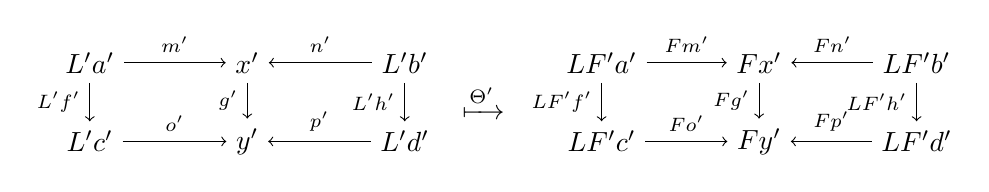
\begin{tikzpicture}
      \begin{scope}
      \node (1) at (-2,1) {\( L'a' \)};
      \node (2) at (0,1) {\( x' \)};
      \node (3) at (2,1) {\( L'b' \)};
      \node (4) at (-2,0) {\( L'c' \)};
      \node (5) at (0,0) {\( y' \)};
      \node (6) at (2,0) {\( L'd' \)};
      \draw [->] (1) to node [above] {\scriptsize{\( m' \)}} (2);
      \draw [->] (3) to node [above] {\scriptsize{\( n' \)}} (2);
      \draw [->] (4) to node [above] {\scriptsize{\( o' \)}} (5);
      \draw [->] (6) to node [above] {\scriptsize{\( p' \)}} (5);
      \draw [->] (1) to node [left] {\scriptsize{\( L'f' \)}} (4);
      \draw [->] (2) to node [left] {\scriptsize{\( g' \)}} (5);
      \draw [->] (3) to node [left] {\scriptsize{\( L'h' \)}} (6);
      \end{scope}
      %
      \begin{scope}[shift={(3,0)}]
      \node (1) at (0,0.5) { $ \xmapsto{ \Theta' } $ };
      \end{scope}
      %
      \begin{scope}[shift={(6.5,0)}]
      \node (1) at (-2,1) {\( LF'a' \)};
      \node (2) at (0,1) {\( Fx' \)};
      \node (3) at (2,1) {\( LF'b' \)};
      \node (4) at (-2,0) {\( LF'c' \)};
      \node (5) at (0,0) {\( Fy' \)};
      \node (6) at (2,0) {\( LF'd' \)};
      \draw [->] (1) to node [above] {\scriptsize{\( Fm' \)}} (2);
      \draw [->] (3) to node [above] {\scriptsize{\( Fn' \)}} (2);
      \draw [->] (4) to node [above] {\scriptsize{\( Fo' \)}} (5);
      \draw [->] (6) to node [above] {\scriptsize{\( Fp' \)}} (5);
      \draw [->] (1) to node [left] {\scriptsize{\( LF'f' \)}} (4);
      \draw [->] (2) to node [left] {\scriptsize{\( Fg' \)}} (5);
      \draw [->] (3) to node [left] {\scriptsize{\( LF'h' \)}} (6);  
      \end{scope}
    \end{tikzpicture}
  \]  
\end{theorem}

\begin{proof}
  In light of Lemma \ref{thm:strcsp-istopos}, it suffices to show that
  $ \Theta \dashv \Theta' $ gives a geometric morphism.

  Denote the structured cospans
  %
  \[
    (m,n) \colon \csp{La}{x}{Lb}
  \]
  % 
  in $ \StrCsp_{ L } $ by $ \ell $ and  
  %
  \[
    (m',n') \colon \csp{L'a'}{x'}{L'b'}
  \]
  % 
  in $ \StrCsp_{ L' } $ by $ \ell' $. Also, denote the unit and counit
  for $F \dashv G$ by $ \eta $, $ \varepsilon $ and for
  $ F' \dashv G' $ by $ \eta' $, $ \varepsilon' $.  The assignments
  %
  \begin{align}
    \left(
      ( f,g,h ) \from \ell \to \Theta' \ell'
      \right)
    & \mapsto
    \left(
      ( \varepsilon' \circ F'f , \varepsilon \circ Fg , \varepsilon'
      \circ F'h )
      \from \Theta \ell \to \ell'
      \right) \\
      %
      \left(
      ( f',g',h' ) \from \Theta \ell \to \ell'
      \right)
    & \mapsto
      \left(
      ( G'f' \circ \eta', Gg' \circ \eta , G'h' \circ \eta' )
      \from \ell \to \Theta' \ell'
      \right) 
  \end{align}
  %
  give a bijection $ \hom ( \Theta \ell , \ell' ) \simeq \hom ( \ell ,
  \Theta' \ell' ) $. Moreover, it is natural in $ \ell $ and $ \ell'
  $. This rests on the natural maps $ \eta $, $ \varepsilon $, $ \eta'
  $, and $ \varepsilon' $. The left adjoint $ \Theta' $ preserves
  finite limits because they are taken pointwise and $ L $, $ F $, and
  $ F' $ all preserve finite limits.
\end{proof}

Even though $ \StrCsp_L $ is a topos, and we are heavily dependent on
the topos theory, we are not currently interested in developing the
theory of stuctured cospans interal to $ \Topos $. The primary reason
is that the sort of morphisms $ \StrCsp_L \to \StrCsp_{L'} $ we are
interested in are not geometric morphisms, but instead are the
following.


\begin{definition} \label{def:str-csp-functor}
  A \defn{structured cospan functor} is a pair of finitely continuous
  and cocontinuous functors $ F \from \X \to \X' $ and
  $ G \from \A \to \A' $ such that $ FL=L'F $ and $ GR = R'F $.
\end{definition}

Structured cospan categories and their morphisms do form a category, but
we leave it unnamed.

% ~~~~~~~~~~~~~~~~~~~~~~~~
% ~~~~~~~~~~~~~~~~~~~~~~~~

\subsection{Structured cospans as arrows}
\label{sec:StrCsp-as-Arrows}

We now turn to capturing the compositional structure that
truly motivates the invention of structured cospans.  To do this, we
shift perspectives from structured cospans as objects in $ \StrCsp_{L} $
to structured cospans as morphisms. 

\begin{definition}
\label{def:strcsp-arr}  
  Denote by $ \Csp_{L} $ the category that has the same objects as
  $ \A $ and structured cospans $ \csp{La}{x}{Lb} $ as arrows of
  type $ a \to b $.
\end{definition}

Note that the composition of $ \csp{La}{x}{Lb} $ with $
\csp{Lb}{y}{Lc} $ is given by pushout:
%
\[
  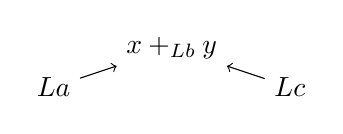
\begin{tikzpicture}
    \begin{scope}[]
    \node (1) at (0,0) {\( La \)};
    \node (2) at (1.5,0.5) {\( x +_{Lb} y \)};
    \node (3) at (3,0) {\( Lc \)};
     \draw [->] (1) to node [] {\scriptsize{\(  \)}} (2);
    \draw [->] (3) to node [] {\scriptsize{\(  \)}} (2); 
    \end{scope}
  \end{tikzpicture}
\]
% 
Pushouts, in a sense, are a way of gluing things together. Hence using
pushouts as composition is a sensible way to model system connection.
The composition above is like connecting along $ Lb $. To illustrate this
we return to the open graphs example.

\begin{example}
\label{ex:open-graph-as-arrow}
  The open graph
  % 
  \[
    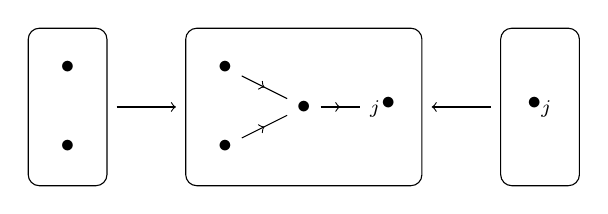
\begin{tikzpicture}
       %
      \begin{scope} % left graph
      \node (1) at (0,1) { \( \bullet \) };
      \node (2) at (0,0) { \( \bullet \) };
      \draw [rounded corners] (-0.5,-0.5) rectangle (0.5,1.5);
      \end{scope}
      %
      \begin{scope}[shift={(2,0)}] % center graph
      \node (1) at (0,1) {\( \bullet \)};
      \node (2) at (0,0) {\( \bullet \)};
      \node (3) at (1,0.5) {\( \bullet  \)};
      \node (4) at (2,0.5) {\( {}_{j} \bullet  \)};
      \draw [->-] (1) to (3);
      \draw [->-] (2) to (3);
      \draw [->-] (3) to (4);
      \draw [rounded corners] (-0.5,-0.5) rectangle (2.5,1.5);
      \end{scope}
      %
      \begin{scope}[shift={(6,0)}] % right graph
      \node (1) at (0,0.5) {\( \bullet_{j} \)};
      \draw [rounded corners] (-0.5,-0.5) rectangle (0.5,1.5);
      \end{scope}
      %
      \begin{scope} % graph morphisms
      \node (1) at (0.5,0.5) {};
      \node (2) at (1.5,0.5) {};
      \node (3) at (4.5,0.5) {};
      \node (4) at (5.5,0.5) {};
      \draw [->] (1) to (2);
      \draw [->] (4) to (3);
      \end{scope}
      %
    \end{tikzpicture}
  \]
  % 
  can be composed with the open graph
   %
  \[
    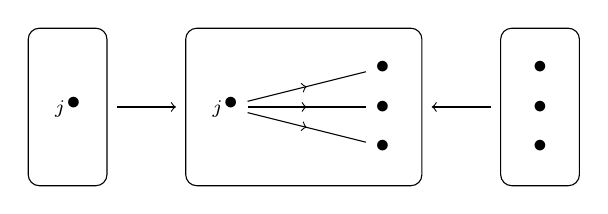
\begin{tikzpicture}
       %
      \begin{scope} % left graph
      \node (1) at (0,0.5) { \( {}_{j} \bullet \) };
      \draw [rounded corners] (-0.5,-0.5) rectangle (0.5,1.5);
      \end{scope}
      %
      \begin{scope}[shift={(2,0)}] % center graph
      \node (1) at (0,0.5) {\( {}_{j} \bullet \)};
      \node (2) at (2,0) {\( \bullet \)};
      \node (3) at (2,0.5) {\( \bullet  \)};
      \node (4) at (2,1) {\( \bullet  \)};
      \draw [->-] (1) to (2);
      \draw [->-] (1) to (3);
      \draw [->-] (1) to (4);
      \draw [rounded corners] (-0.5,-0.5) rectangle (2.5,1.5);
      \end{scope}
      %
      \begin{scope}[shift={(6,0)}] % right graph
      \node (2) at (0,0) {\( \bullet \)};
      \node (3) at (0,0.5) {\( \bullet  \)};
      \node (4) at (0,1) {\( \bullet  \)};
      \draw [rounded corners] (-0.5,-0.5) rectangle (0.5,1.5);
      \end{scope}
      %
      \begin{scope} % graph morphisms
      \node (1) at (0.5,0.5) {};
      \node (2) at (1.5,0.5) {};
      \node (3) at (4.5,0.5) {};
      \node (4) at (5.5,0.5) {};
      \draw [->] (1) to (2);
      \draw [->] (4) to (3);
      \end{scope}
      %
    \end{tikzpicture}
  \]
  %
  to obtain
  %
  \[
    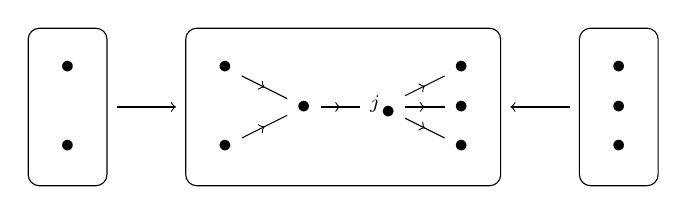
\begin{tikzpicture}
       %
      \begin{scope} % left graph
      \node (1) at (0,1) { \( \bullet \) };
      \node (2) at (0,0) { \( \bullet \) };
      \draw [rounded corners] (-0.5,-0.5) rectangle (0.5,1.5);
      \end{scope}
      %
      \begin{scope}[shift={(2,0)}] % center graph
      \node (1) at (0,1) {\( \bullet \)};
      \node (2) at (0,0) {\( \bullet \)};
      \node (3) at (1,0.5) {\( \bullet  \)};
      \node (4) at (2,0.5) {\( {}^{j} \bullet  \)};
      \node (5) at (3,0) {\( \bullet \)};
      \node (6) at (3,0.5) {\( \bullet  \)};
      \node (7) at (3,1) {\( \bullet  \)};
      \draw [->-] (1) to (3);
      \draw [->-] (2) to (3);
      \draw [->-] (3) to (4);
      \draw [->-] (4) to (5);
      \draw [->-] (4) to (6);
      \draw [->-] (4) to (7);
      \draw [rounded corners] (-0.5,-0.5) rectangle (3.5,1.5);
      \end{scope}
      %
      \begin{scope}[shift={(7,0)}] % right graph
      \node (2) at (0,0) {\( \bullet \)};
      \node (3) at (0,0.5) {\( \bullet  \)};
      \node (4) at (0,1) {\( \bullet  \)};
      \draw [rounded corners] (-0.5,-0.5) rectangle (0.5,1.5);
      \end{scope}
      %
      \begin{scope} % graph morphisms
      \node (1) at (0.5,0.5) {};
      \node (2) at (1.5,0.5) {};
      \node (3) at (5.5,0.5) {};
      \node (4) at (6.5,0.5) {};
      \draw [->] (1) to (2);
      \draw [->] (4) to (3);
      \end{scope}
      %
    \end{tikzpicture}
  \]
  %
  This composition glued the two open graphs together along the node $
  j $.
  
\end{example}

% ~~~~~~~~~~~~~~~~~~~~~~~~
% ~~~~~~~~~~~~~~~~~~~~~~~~

\subsection{A double category of structured cospans}
\label{sec:DblCatOfStrCsp}

Using double categories allows us to combine into a single instrument
the competing perspectives of structured cospans as objects and as
morphisms. For a precise definition of a symmetric monoidal double
category, we point to Shulman \cite{ShulDblCat}, though for the sake
of completeness, we list the key pieces. A (psuedo) double category
$ \CCC $ is a category weakly internal to $ \Cat $. Roughly, this is a
pair of categories $ ( \C_0 , \C_1 ) $ assembled together as follows.
% 
\begin{itemize}
\item The $ \CCC $-objects are exactly the $ \C_0 $-objects.
\item The vertical arrows $ c \to d $ in $ \CCC $ between $ \C
  $-objects are exactly the $ \C_0 $-arrows.
\item The horizontal arrows $ c \horarrow d $ in $ \CCC $ between
  $ \CCC $-objects are $ \C_1 $-objects. 
\item The squares of $ \CCC $ are
\[
  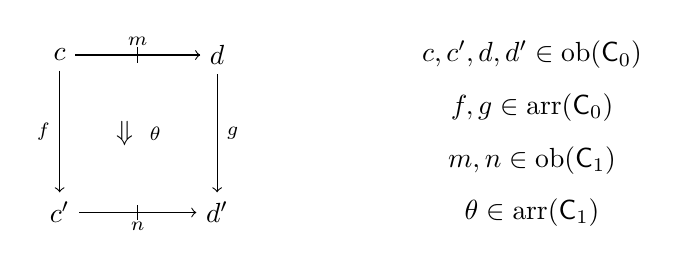
\begin{tikzpicture}
    \node (1) at (0,2) {\( c \)};
    \node (2) at (2,2) {\( d \)};
    \node (3) at (0,0) {\( c' \)};
    \node (4) at (2,0) {\( d' \)};
    \draw [-|->] (1) to node [above] {\scriptsize{\( m \)}} (2);
    \draw [->] (1) to node [left] {\scriptsize{\( f \)}} (3);
    \draw [->] (2) to node [right] {\scriptsize{\( g \)}} (4);
    \draw [-|->] (3) to node [below] {\scriptsize{\( n \)}} (4);
    \node (5) at (6,2) {\( c,c',d,d' \in \operatorname{ob} ( \C_0 ) \)};
    \node (6) at (6,1.33) {\( f,g \in \operatorname{arr} ( \C_0 ) \)};
    \node (7) at (6,.66) {\( m,n \in \operatorname{ob} ( \C_1 ) \)};
    \node (8) at (1,1) {\( \Downarrow \) \scriptsize{ \( \theta \)}};
    \node (9) at (6,0) {\( \theta \in \operatorname{arr} ( \C_1 ) \)};
  \end{tikzpicture}
\]
are the arrows of $ \C_1 $. 
\end{itemize}
%
In addition, there are structure maps ensuring the correct interplay
between the elements of this data.  The vertical arrows compose as
they do in $ \C_0 $ and there is a structure map for composing
horizontal arrows. The squares can compose both horizontally and
vertically.

Observe that the horizontal arrows play two roles: as objects in their
origin category and arrows in the double category. This reflects the
content of the categories $ \StrCsp_{L} $ and $ \Csp_{L} $. Here is a
first example of a double category.

\begin{definition}
  There is a double category
  $ \SSStrCsp_L \coloneqq ( \A , \StrCsp_{L} ) $ :
  \begin{itemize}
  \item the objects are the $ \A $-objects
  \item the vertical arrows $ a \to b $ the $ \A $-arrows, 
  \item the horizontal arrows $ a \horarrow b $ are the cospans
    $ \csp{La}{x}{Lb} $, and
  \item the squares are the commuting diagrams
    %
    \[
    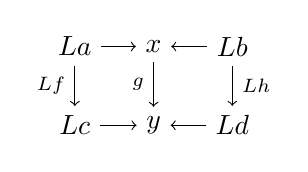
\begin{tikzpicture}
    \node (1) at (0,1) {\( La \)};
    \node (2) at (1,1) {\( x \)};
    \node (3) at (2,1) {\( Lb \)};
    \node (4) at (0,0) {\( Lc \)};
    \node (5) at (1,0) {\( y \)};
    \node (6) at (2,0) {\( Ld \)};
    \draw [->] (1) to node [] {\scriptsize{\(   \)}} (2);
    \draw [->] (3) to node [] {\scriptsize{\(  \)}} (2);
    \draw [->] (4) to node [] {\scriptsize{\(  \)}} (5);
    \draw [->] (6) to node [] {\scriptsize{\(  \)}} (5);
    \draw [->] (1) to node [left] {\scriptsize{\( Lf \)}} (4);
    \draw [->] (2) to node [left] {\scriptsize{\( g \)}} (5);
    \draw [->] (3) to node [right] {\scriptsize{\( Lh \)}} (6);
    \end{tikzpicture}
  \]
  \end{itemize}
  %  
\end{definition}

Baez and Courser proved that this actually is a double category
\cite[Cor.~3.9]{StrCsp}. Moreover, when $ \cat{ A } $ and
$ \cat{ X } $ are cocartesian, their coproducts can be used to define
a tensor product on $ \SSStrCsp_L $. This tensor encodes the idea that
the disjoint union of considering the disjoint union of two systems as
a single system. Because we have no need for this structure in this
paper, we say no more about it.

\begin{remark}
  Double categories are a nice way of capturing both the object-ness
  and arrow-ness of structured cospans.  An alternative would be to
  use bicategories, but this doesn't reflect the nature of structured
  cospans as faithfully as does double categories.
\end{remark}

% ~~~~~~~~~~~~~~~~~~~~~~~~~~~~~~~~~~~~~~~~
% ~~~~~~~~~~~ rewriting ~~~~~~~~~~~~~~~~~~
% ~~~~~~~~~~~~~~~~~~~~~~~~~~~~~~~~~~~~~~~~

\section{Rewriting}
\label{sec:rewriting}

We begin this final section by recalling the basics of double pushout
rewriting within the context of topoi. We also present the second of
our main results: a generalization, from rewriting graphs to rewriting
topoi, about the expressiveness of certain graph grammars.  We then
apply this rewriting theory to structured cospans. In doing so, we
introduce some new categorical bookkeeping devices that shows that the
rewrite relation is obtained functorially. This section contains our
main result which is a generalization of work by Gadducci and Heckle
\cite{Gadd_IndGraphTrans}.  However, this result is not simply a mere
generalization but justifies the study of systems using structured
cospans.  We end the section by exploring this justification.

Double pushout rewriting was introduced for graphs by Ehrig, et.~al.\
\cite{Ehrig_GraphGram}. It has since undergone extensive study and
generalization. Currently, the most general setting to contain a rich
theory of rewriting is adhesive categories, introduced by Lack and
Soboci\'{n}ski \cite{LackSobo_Adhesive}. Topoi, such as structured
cospan categories, are examples of adhesive categories
\cite{LackSobo_ToposIsAdh} so the theory we are developing in this
paper admits rewriting.

Because topoi are the greatest level of generality we need, we only
recall rewriting at this level.  Of course, these concepts hold for
adhesive categories in general, but restricting to topoi allows us to
avoid an unessecary digression 


\subsection{Rewriting topoi}
\label{sec:Adhesive-Rewriting}


Fix a topos $ \C $. Since rewriting in topoi is abstracted
from graph rewriting, the archetypal topos for us is $ \RGraph $.

Rewriting starts with the notion of a \defn{rewrite rule}, or simply
\defn{rule}.  This is a span
%
\[
  \ell \monicgets k \monicto r
\]
% 
in $ \C $ with monic legs. We continue to denote spans by
$ \spn{\ell}{k}{r} $ and specifying it is a rule indicates that the
legs are monic. The conciept of a rule is that $ \ell $ is replaced by
$ r $ with $ k $ a fixed subobject common to both. We can then apply
this rule to suitable objects having $ \ell $ as a subobject.
Suitability for $ m \from \ell \monicto g $ means a
\defn{pushout complement} exists, that is an object $ d $ fitting into a
pushout diagram
%
\[
  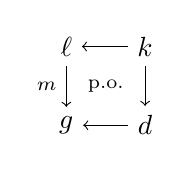
\begin{tikzpicture}
    \node (l) at (0,1) {$ \ell $};
    \node (k) at (1,1) {$ k $};
    \node (g) at (0,0) {$ g $};
    \node (d) at (1,0) {$ d $};
    \draw [->] (k) to node [] {\scriptsize{$  $}} (l);
    \draw [->] (d) to node [] {\scriptsize{$  $}} (g);
    \draw [->] (l) to node [left] {\scriptsize{$ m $}} (g);
    \draw [->] (k) to node [] {\scriptsize{$  $}} (d);
    \node () at (0.5,0.5) {\scriptsize{p.o.}};
  \end{tikzpicture}
\]
% 
A pushout complement need not exist, but if it does
and the map $ k \to \ell $ is monic, then it is unique up to
isomorphism \cite[Lem.~15]{LackSobo_Adhesive}. Given a rule together
with a suitable $ g $, we obtain a \defn{derived rule} on the bottom
row of the \emph{double pushout diagram}
%
\[
  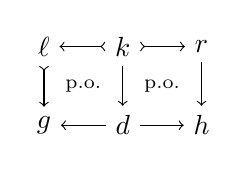
\begin{tikzpicture}
    \node (1) at (0,1) {$ \ell $};
    \node (2) at (1,1) {$ k $};
    \node (3) at (2,1) {$ r $};
    \node (4) at (0,0) {$ g $};
    \node (5) at (1,0) {$ d $};
    \node (6) at (2,0) {$ h $};
    \draw [>->] (2) to node [] {\scriptsize{$  $}} (1);
    \draw [>->] (2) to node [] {\scriptsize{$  $}} (3);
    \draw [->] (5) to node [] {\scriptsize{$  $}} (4);
    \draw [->] (5) to node [] {\scriptsize{$  $}} (6);
    \draw [>->] (1) to node [] {\scriptsize{$  $}} (4);
    \draw [->] (2) to node [] {\scriptsize{$  $}} (5);
    \draw [->] (3) to node [] {\scriptsize{$  $}} (6);
    \node () at (0.5,0.5) {\scriptsize{p.o.}};
    \node () at (1.5,0.5) {\scriptsize{p.o.}};
  \end{tikzpicture}
\]
%
Indeed, the span $ \spn{g}{d}{h} $ is a rule because pushouts preserve
monics in topoi \cite[Lem.~12]{LackSobo_Adhesive}. The intuition of
this is that we are identifying an instance of $ \ell $ in $ g $ and
replacing it with $ r $ in a cohesive manner, thus resulting in a new
object $ h $.  

A topos $ \C $ together with a finite set $ P $ of rules
$ \{ \spn{\ell_j}{k_j}{r_j} \} $ in $ \cat{ C } $ is called a
\defn{grammar}. An arrow of grammars $ ( \C , P ) \to ( \D , Q ) $ is
a generic functor $ F \from \C \to \D $ such that
$ FP \subseteq Q $. Together these form a category $ \Gram $.

Every grammar $ ( \C , P ) $ gives rise to a relation on the objects
of $ \C $ defined by $ \dderiv{g}{h} $ whenever there exists a rule
$ \spn{g}{d}{h} $ derived from a production in $ P $. However, this
relation is not sufficient.  For one, it is not true in general that
$ \dderiv{x}{x} $ holds. Also, it doesn't capture multistep
rewrites. That is, perhaps there are derived rules witnessing
$ \dderiv{g}{g'} $ and $ \dderiv{g'}{g''} $ but not a derived rule
witnessing $ \dderiv{g}{g''} $. However, we want to be able to relate
a pair of objects if one can be rewritten into another after a finite
sequence of derived rules. Therefore, the relation we actually want is
the reflexive and transitive closure of $ \rightsquigarrow $, which we
denote by $ \rightsquigarrow^\ast $.  This is called the \defn{rewrite
  relation}.  Every grammar gives rise to a unique rewrite
relation. Moreover, this can be done functorially, though we content
ourselves to restrict our attention to showing this in the context of
structured cospan categories.

\subsection{Generalizing a result from graph rewriting}
\label{sec:gen-result-graph-rewriting}

In this section, we lift a well-known result
\cite[Prop.~3.3]{Ehrig_GraphGram} from the theory of rewriting graphs
into the theory of rewriting topoi. 

The original result is as follows.  Let
$ \flat \from \RGraph \to \RGraph $ denote the underlying discrete
graph comonad. Given a grammar $ ( \RGraph , P ) $, define a new
grammar $ ( \RGraph , P_\flat ) $ where $ P_\flat $ consists of rules
$ k_\flat \hookrightarrow k \to \ell \times r $ for each rule
$ \spn{\ell}{k}{r} $ in $ P $. Then a graph $ g $ is related to a
graph $ h $ with respect to the rewrite relation induced by
$ ( \RGraph , P ) $ if and only if $ g $ is related to $ h $ with
respect to the rewriting relation induced by
$ ( \RGraph , P_\flat ) $.

To generalize this result, we first need a few notions.  Fix a
geometric morphism $ L \dashv R \from \X \to \A $. Denote by
$ ( \X , P_\flat ) $ the \defn{discrete grammar} underlying
$ ( \X , P ) $. This consists of all rules obtained by pulling back
$ k \to \ell \times r $ by the counit $ LRk \to k $ for each rule in
$ P $.

Recall that a poset is \textbf{well-founded} if every non-empty subset
has a minimal element.  Whenever the axiom of choice is present,
well-foundedness is equivalent to the lack of infinite descending
chains. For a relevant example, as the axiom of choice holds in any
presheaf category, the Heyting algebra $ \Sub ( x ) $ for any
finite-set valued presheaf $ x $ is well-founded.

\begin{theorem}
\label{thm:production-same-rewrite-relation-as-discrete}
Fix a geometric morphism $ L \dashv R \from \X \to \A $ with monic
counit. Let $ ( \X , P ) $ be a grammar such that for every
$ \X $-object $ x $ in the apex of a production of $ P $, the Heyting
algebra $ \Sub (x) $ is well-founded.  The rewriting relation for a
grammar $ ( \X , P ) $ is equal to rewriting relation for the grammar
$ ( \X , P_{\flat} ) $
\end{theorem}

\begin{proof}
  For any derivation
  %
  \[
  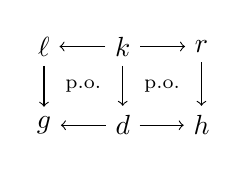
\begin{tikzpicture}
    \node (1t) at (0,1) {$ \ell $};
    \node (2t) at (1,1) {$ k $};
    \node (3t) at (2,1) {$ r $};
    \node (1b) at (0,0) {$ g $};
    \node (2b) at (1,0) {$ d $};
    \node (3b) at (2,0) {$ h $};
    \draw [->] (2t) to node [] {\scriptsize{$  $}} (1t);
    \draw [->] (2t) to node [] {\scriptsize{$  $}} (3t);
    \draw [->] (2b) to node [] {\scriptsize{$  $}} (1b);
    \draw [->] (2b) to node [] {\scriptsize{$  $}} (3b);
    \draw [->] (1t) to node [] {\scriptsize{$  $}} (1b);
    \draw [->] (2t) to node [] {\scriptsize{$  $}} (2b);
    \draw [->] (3t) to node [] {\scriptsize{$  $}} (3b);
    \node () at (0.5,0.5) {\scriptsize{p.o.}};
    \node () at (1.5,0.5) {\scriptsize{p.o.}};
  \end{tikzpicture}
  \]
  % 
  arising from $ P $, there is a derivation
  %
  \[
  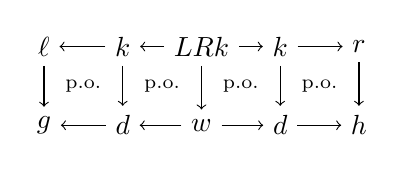
\begin{tikzpicture}
    \node (01) at (0,1) {$ \ell $};
    \node (11) at (1,1) {$ k $};
    \node (21) at (2,1) {$ LRk $};
    \node (31) at (3,1) {$ k $};
    \node (41) at (4,1) {$ r $};
    \node (00) at (0,0) {$ g $};
    \node (10) at (1,0) {$ d $};
    \node (20) at (2,0) {$ w $};
    \node (30) at (3,0) {$ d $};
    \node (40) at (4,0) {$ h $};
    \draw [->] (11) to node [] {\scriptsize{$  $}} (01);
    \draw [->] (21) to node [] {\scriptsize{$  $}} (11);
    \draw [->] (21) to node [] {\scriptsize{$  $}} (31);
    \draw [->] (31) to node [] {\scriptsize{$  $}} (41);
    \draw [->] (10) to node [] {\scriptsize{$  $}} (00);
    \draw [->] (20) to node [] {\scriptsize{$  $}} (10);
    \draw [->] (20) to node [] {\scriptsize{$  $}} (30);
    \draw [->] (30) to node [] {\scriptsize{$  $}} (40);
    \draw [->] (01) to node [] {\scriptsize{$  $}} (00);
    \draw [->] (11) to node [] {\scriptsize{$  $}} (10);
    \draw [->] (21) to node [] {\scriptsize{$  $}} (20);
    \draw [->] (31) to node [] {\scriptsize{$  $}} (30);
    \draw [->] (41) to node [] {\scriptsize{$  $}} (40);
    \node () at (0.5,0.5) {\scriptsize{p.o.}};
    \node () at (1.5,0.5) {\scriptsize{p.o.}};
    \node () at (2.5,0.5) {\scriptsize{p.o.}};
    \node () at (3.5,0.5) {\scriptsize{p.o.}};
  \end{tikzpicture}
  \]
  %
  where 
  %
  \[
    w \coloneqq
    \bigwedge \{ z \colon z \wedge k = x \} \vee LRk.
  \]
  Note that $ w \vee k = x $ and $ w \wedge k = LRy $ which gives that
  the two inner squares of the lower diagram are pushouts.
\end{proof}

% % ~~~~~~~~~~~~~~~~~~~~~~~~
% % ~~~~~~~~~~~~~~~~~~~~~~~~

\subsection{Rewriting structured cospans}
\label{sec:Rewriting-StrCsp}

We now turn to rewriting structured cospans. The ability of structured
cospans to give a nice theory of rewriting lies in the fact that they
form a topos (Theorem \ref{thm:strcsp-istopos}).  The first thing we
do is appropriately restrict $ \Gram $ to a subcategory
$ \StrCspGram $.  The objects are $ ( \StrCsp_{L} , P ) $ where $ P $
consists of rules of the form
 %
 \[
   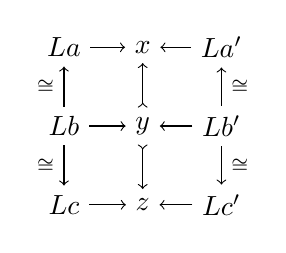
\begin{tikzpicture}
    \begin{scope}
        \node (1) at (0,2) {\( La \)};
        \node (2) at (1,2) {\( x \)};
        \node (3) at (2,2) {\( La' \)};
        \node (4) at (0,1) {\( Lb \)};
        \node (5) at (1,1) {\( y \)};
        \node (6) at (2,1) {\( Lb' \)};
        \node (7) at (0,0) {\( Lc \)};
        \node (8) at (1,0) {\( z \)};
        \node (9) at (2,0) {\( Lc' \)};
        \draw [->] (1) to node []
          {\scriptsize{\( \)}} (2);
        \draw [->] (3) to node []
          {\scriptsize{\( \)}} (2);
        \draw [->] (4) to node []
          {\scriptsize{\( \)}} (5);
        \draw [->] (6) to node []
          {\scriptsize{\( \)}} (5);
        \draw [->] (7) to node []
          {\scriptsize{\( \)}} (8);
        \draw [->] (9) to node []
          {\scriptsize{\( \)}} (8);
        \draw [->] (4) to node [left]
          {\scriptsize{\( \iso \)}} (1);
        \draw [->] (4) to node [left]
          {\scriptsize{\( \iso \)}} (7);
        \draw [>->] (5) to node []
          {\scriptsize{\( \)}} (2);
        \draw [>->] (5) to node []
          {\scriptsize{\( \)}} (8);
        \draw [->] (6) to node [right]
          {\scriptsize{\( \iso \)}} (3);
        \draw [->] (6) to node [right]
          {\scriptsize{\( \iso \)}} (9);
    \end{scope}
  \end{tikzpicture}
\]
%
and the morphisms are the structured cospan functors (Definition
\ref{def:str-csp-functor}) that are stable under the grammars.

Recall that to each grammar is associated a relation
$ \rightsquigarrow $ and its reflexive transitive closure, the rewrite
relation$ \rightsquigarrow^\ast $. We now show that this can be done
functorially via a composite of two functors,
$ D \from \StrCspGram \to \StrCspGram $ and
$ S \from \StrCspGram \to \DblCat $, which we now define.

\todo{is composition preserved?}

\begin{lemma}
  There is an idempotent functor
  $ D \from \StrCspGram \to \StrCspGram $. It is defined on objects by
  setting $ D ( \StrCsp_L , P ) $ to be the grammar
  $ ( \StrCsp_L , P') $, where $ P' $ consists of all rules
  $ \spn{g}{h}{d} $ witnessing the relation $ \dderiv{g}{h} $ with
  respect to $ ( \StrCsp_L , P ) $. On arrows,
  $ DF \from D( \StrCsp_K , P ) \to D( \StrCsp_L , Q ) $ is defined
  exactly as $ F $.  Moreover, the identity on $ \StrCspGram $ is a
  subfunctor of $ D $.
\end{lemma}

\begin{proof}
  That $ D ( \StrCsp , P ) $ actually gives a grammar follows from the
  fact that pushouts respect monics in a topos
  \cite[Lem.~12]{LackSobo_Adhesive}.
  
  That $ D $ is idempotent is equivalent to saying that, for a set
  $ P $ of rules, $ \dderiv{g}{h} $ with respect to
  $ D ( \StrCsp_LGram , P ) $ if and only if $ \dderiv{g}{h} $ with
  respect to $ DD ( \StrCspGram_L , P ) $. This follows from the fact
  that the outer box of the diagram
    %
    \[
      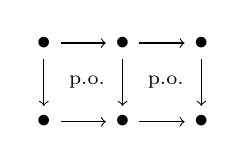
\begin{tikzpicture}
        \node (1) at (0,1) {\( \bullet \)};
        \node (2) at (1,1) {\( \bullet \)};
        \node (3) at (2,1) {\( \bullet \)};
        \node (4) at (0,0) {\( \bullet \)};
        \node (5) at (1,0) {\( \bullet \)};
        \node (6) at (2,0) {\( \bullet \)};
        \draw [->] (1) to node [] {\scriptsize{\(  \)}} (2);
        \draw [->] (2) to node [] {\scriptsize{\(  \)}} (3);
        \draw [->] (4) to node [] {\scriptsize{\(  \)}} (5);
        \draw [->] (5) to node [] {\scriptsize{\(  \)}} (6);
        \draw [->] (1) to node [] {\scriptsize{\(  \)}} (4);
        \draw [->] (2) to node [] {\scriptsize{\(  \)}} (5);
        \draw [->] (3) to node [] {\scriptsize{\(  \)}} (6);
        \node () at (0.5,0.5) {\scriptsize{ p.o.\ }};
        \node () at (1.5,0.5) {\scriptsize{ p.o.\ }};
      \end{tikzpicture}
    \]
    %
    is a pushout.

    The identity is a subfunctor of $ D $ because $ \dderiv{\ell}{r} $
    for any production $ \spn{\ell }{k}{r} $ in $ ( \StrCsp_L , P ) $
    via a triple of identity arrows. Hence the identity functor on
    $ \StrCsp_L $ turns $ ( \StrCsp_L , P ) $ into a subobject of
    $ D ( \StrCsp_L , P ) $.
\end{proof}

\todo{what's the meaning of this lemma?}

To define $ S $, we reference the double category $ \MonSpCsp (\C) $
for a topos $ \C $ introduced in \cite{CicCour_SpCspTopos}.  The
objects are those in $ \C $, the vertical arrows are spans with
invertible legs in $ \C $, the horizontal arrows are cospans in
$ \C $, and the squares are diagrams in $ \C $ with shape
%
\[
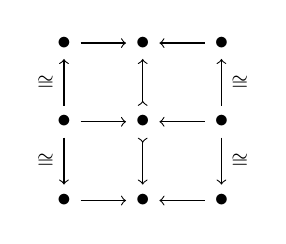
\begin{tikzpicture}
  \node (00) at (0,0) {$ \bullet $};
  \node (01) at (0,1) {$ \bullet $};
  \node (02) at (0,2) {$ \bullet $};
  \node (10) at (1,0) {$ \bullet $};
  \node (11) at (1,1) {$ \bullet $};
  \node (12) at (1,2) {$ \bullet $};
  \node (20) at (2,0) {$ \bullet $};
  \node (21) at (2,1) {$ \bullet $};
  \node (22) at (2,2) {$ \bullet $};
  \draw [->] (02) to node [] {\scriptsize{$  $}} (12);
  \draw [->] (22) to node [] {\scriptsize{$  $}} (12);
  \draw [->] (01) to node [] {\scriptsize{$  $}} (11);
  \draw [->] (21) to node [] {\scriptsize{$  $}} (11);
  \draw [->] (00) to node [] {\scriptsize{$  $}} (10);
  \draw [->] (20) to node [] {\scriptsize{$  $}} (10);
  \draw [->] (01) to node [left] {\scriptsize{$ \cong  $}} (02);
  \draw [->] (01) to node [left] {\scriptsize{$ \cong $}} (00);
  \draw [>->] (11) to node [] {\scriptsize{$  $}} (12);
  \draw [>->] (11) to node [] {\scriptsize{$  $}} (10);
  \draw [->] (21) to node [right] {\scriptsize{$ \cong $}} (22);
  \draw [->] (21) to node [right] {\scriptsize{$ \cong $}} (20);
\end{tikzpicture}
\]
%

Given a structured cospan grammar $ ( \StrCsp_L , P ) $, observe that
the productions in $ P $ are admissible as squares in
$ \MonSpCsp (\X) $. Denote by $ S ( \StrCsp_L , P ) $ the sub-double
category of $ \MonSpCsp ( \X ) $ that is full on objects, vertical and
horizontal arrows, and generated by the productions in
$ P $. This assignment is functorial
%
\todo{double check this}
%
because
%
\[
  (F,G) \from ( \StrCsp_{L} , P ) \to ( \StrCsp_{L'} , P' )
\]
% 
gives a mapping between the generators of $ S ( \StrCsp_{L} , P ) $
and $ S ( \StrCsp_{L'} , P' ) $.  Composition holds because
$ F $ and $ G $ both preserve pullbacks and pushouts. This allows
us to define the language functor $ \Lang \coloneqq SD $.  

%
\todo{ rotate to main result }
% 


Here is a quick lemma that we use in the next theorm.

\begin{lemma}
\label{thm:rewrite-rel-is-additive}
  If $ \deriv{x}{y} $ and $ \deriv{x'}{y'} $, then $ \deriv{x+x'}{y+y'} $
\end{lemma}

\begin{proof}
  It the derivation $ \deriv{x}{y} $ comes from a string of double
  pushout diagrams
  %
  \[
    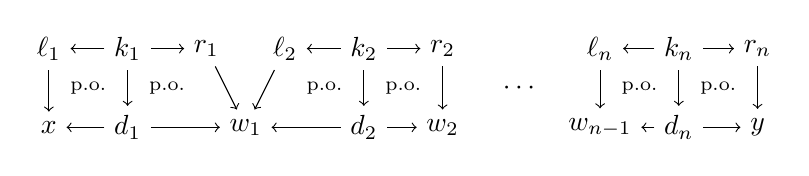
\begin{tikzpicture}
      \node (1t) at (0,1) {$ \ell_1 $};
      \node (2t) at (1,1) {$ k_1 $};
      \node (3t) at (2,1) {$ r_1 $};
      \node (4t) at (3,1) {$ \ell_2 $};
      \node (5t) at (4,1) {$ k_2 $};
      \node (6t) at (5,1) {$ r_2 $};
      \node (7t) at (7,1) {$ \ell_n $};
      \node (8t) at (8,1) {$ k_n $};
      \node (9t) at (9,1) {$ r_n $};
      \node (1b) at (0,0) {$ x $};
      \node (2b) at (1,0) {$ d_1 $};
      \node (3b) at (2.5,0) {$ w_1 $};
      \node (4b) at (4,0) {$ d_2 $};
      \node (5b) at (5,0) {$ w_2 $};
      \node (6b) at (7,0) {$ w_{n-1} $};
      \node (7b) at (8,0) {$ d_n $};
      \node (8b) at (9,0) {$ y $};
      \draw [->] (2t) to node [] {\scriptsize{$  $}} (1t);
      \draw [->] (2t) to node [] {\scriptsize{$  $}} (3t);
      \draw [->] (5t) to node [] {\scriptsize{$  $}} (4t);
      \draw [->] (5t) to node [] {\scriptsize{$  $}} (6t);
      \draw [->] (8t) to node [] {\scriptsize{$  $}} (7t);
      \draw [->] (8t) to node [] {\scriptsize{$  $}} (9t);
      \draw [->] (2b) to node [] {\scriptsize{$  $}} (1b);
      \draw [->] (2b) to node [] {\scriptsize{$  $}} (3b);
      \draw [->] (4b) to node [] {\scriptsize{$  $}} (3b);
      \draw [->] (4b) to node [] {\scriptsize{$  $}} (5b);
      \draw [->] (7b) to node [] {\scriptsize{$  $}} (6b);
      \draw [->] (7b) to node [] {\scriptsize{$  $}} (8b);
      \draw [->] (1t) to node [] {\scriptsize{$  $}} (1b);
      \draw [->] (2t) to node [] {\scriptsize{$  $}} (2b);
      \draw [->] (3t) to node [] {\scriptsize{$  $}} (3b);
      \draw [->] (4t) to node [] {\scriptsize{$  $}} (3b);
      \draw [->] (5t) to node [] {\scriptsize{$  $}} (4b);
      \draw [->] (6t) to node [] {\scriptsize{$  $}} (5b);
      \draw [->] (7t) to node [] {\scriptsize{$  $}} (6b);
      \draw [->] (8t) to node [] {\scriptsize{$  $}} (7b);
      \draw [->] (9t) to node [] {\scriptsize{$  $}} (8b);
      \node () at (6,0.5) {$ \dotsm $};
      \node () at (0.5,0.5) {\scriptsize{p.o.}};
      \node () at (1.5,0.5) {\scriptsize{p.o.}};
      \node () at (3.5,0.5) {\scriptsize{p.o.}};
      \node () at (4.5,0.5) {\scriptsize{p.o.}};
      \node () at (7.5,0.5) {\scriptsize{p.o.}};
      \node () at (8.5,0.5) {\scriptsize{p.o.}};
    \end{tikzpicture}
  \]
  %
  and the derivation $ \deriv{x}{y} $ comes from a string of double
  pushout diagrams
  %
  \[
    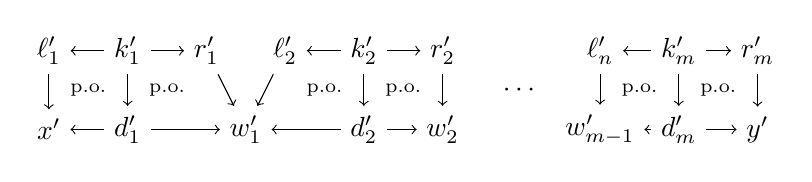
\begin{tikzpicture}
      \node (1t) at (0,1) {$ \ell'_1 $};
      \node (2t) at (1,1) {$ k'_1 $};
      \node (3t) at (2,1) {$ r'_1 $};
      \node (4t) at (3,1) {$ \ell'_2 $};
      \node (5t) at (4,1) {$ k'_2 $};
      \node (6t) at (5,1) {$ r'_2 $};
      \node (7t) at (7,1) {$ \ell'_n $};
      \node (8t) at (8,1) {$ k'_m $};
      \node (9t) at (9,1) {$ r'_m $};
      \node (1b) at (0,0) {$ x' $};
      \node (2b) at (1,0) {$ d'_1 $};
      \node (3b) at (2.5,0) {$ w'_1 $};
      \node (4b) at (4,0) {$ d'_2 $};
      \node (5b) at (5,0) {$ w'_2 $};
      \node (6b) at (7,0) {$ w'_{m-1} $};
      \node (7b) at (8,0) {$ d'_m $};
      \node (8b) at (9,0) {$ y' $};
      \draw [->] (2t) to node [] {\scriptsize{$  $}} (1t);
      \draw [->] (2t) to node [] {\scriptsize{$  $}} (3t);
      \draw [->] (5t) to node [] {\scriptsize{$  $}} (4t);
      \draw [->] (5t) to node [] {\scriptsize{$  $}} (6t);
      \draw [->] (8t) to node [] {\scriptsize{$  $}} (7t);
      \draw [->] (8t) to node [] {\scriptsize{$  $}} (9t);
      \draw [->] (2b) to node [] {\scriptsize{$  $}} (1b);
      \draw [->] (2b) to node [] {\scriptsize{$  $}} (3b);
      \draw [->] (4b) to node [] {\scriptsize{$  $}} (3b);
      \draw [->] (4b) to node [] {\scriptsize{$  $}} (5b);
      \draw [->] (7b) to node [] {\scriptsize{$  $}} (6b);
      \draw [->] (7b) to node [] {\scriptsize{$  $}} (8b);
      \draw [->] (1t) to node [] {\scriptsize{$  $}} (1b);
      \draw [->] (2t) to node [] {\scriptsize{$  $}} (2b);
      \draw [->] (3t) to node [] {\scriptsize{$  $}} (3b);
      \draw [->] (4t) to node [] {\scriptsize{$  $}} (3b);
      \draw [->] (5t) to node [] {\scriptsize{$  $}} (4b);
      \draw [->] (6t) to node [] {\scriptsize{$  $}} (5b);
      \draw [->] (7t) to node [] {\scriptsize{$  $}} (6b);
      \draw [->] (8t) to node [] {\scriptsize{$  $}} (7b);
      \draw [->] (9t) to node [] {\scriptsize{$  $}} (8b);
      \node () at (6,0.5) {$ \dotsm $};
      \node () at (0.5,0.5) {\scriptsize{p.o.}};
      \node () at (1.5,0.5) {\scriptsize{p.o.}};
      \node () at (3.5,0.5) {\scriptsize{p.o.}};
      \node () at (4.5,0.5) {\scriptsize{p.o.}};
      \node () at (7.5,0.5) {\scriptsize{p.o.}};
      \node () at (8.5,0.5) {\scriptsize{p.o.}};
    \end{tikzpicture}
  \]
  % 
  then $ \deriv{x+x'}{y+y'} $ is realized by concatenating to the end
  of first string with $ x' $ summed with the bottom row the second
  string with $ y $ summed on the bottom row.
\end{proof}

The desire behind the main result is the ability to study systems, as
represented by objects in a topos $ \X $, locally.  The mechanism
(that is, structured cospans) by which we do this is to equip systems
with interfaces that allow us to connect sub-systems together. Another
way to view this is that given a system can be decomposed into
sub-systems. These can be studied individually then reconnected along
the interfaces this mechanism provides. The manner in which the
main result can accomplish this is discussed below the theorem

We need the following definition. Associate to a grammar
$ ( \X , P ) $ the structured cospan grammar $ ( \StrCsp_L , P' ) $
where $ P' $ contains
%
\[
  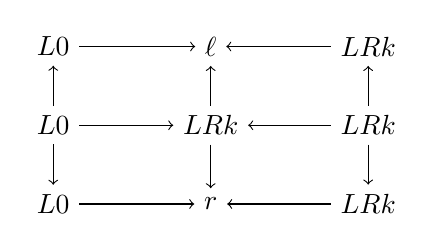
\begin{tikzpicture}
    \node (1) at (0,2) {$ L 0 $};
    \node (2) at (2,2) {$ \ell $};
    \node (3) at (4,2) {$ LRk $};
    \node (4) at (0,1) {$ L 0 $};
    \node (5) at (2,1) {$ LRk $};
    \node (6) at (4,1) {$ LRk $};
    \node (7) at (0,0) {$ L 0 $};
    \node (8) at (2,0) {$ r $};
    \node (9) at (4,0) {$ LRk $};
    \draw [->] (1) to node [] {\scriptsize{$  $}} (2);
    \draw [->] (3) to node [] {\scriptsize{$  $}} (2);
    \draw [->] (4) to node [] {\scriptsize{$  $}} (5);
    \draw [->] (6) to node [] {\scriptsize{$  $}} (5);
    \draw [->] (7) to node [] {\scriptsize{$  $}} (8);
    \draw [->] (9) to node [] {\scriptsize{$  $}} (8);
    \draw [->] (4) to node [] {\scriptsize{$  $}} (1);
    \draw [->] (4) to node [] {\scriptsize{$  $}} (7);
    \draw [->] (5) to node [] {\scriptsize{$  $}} (2);
    \draw [->] (5) to node [] {\scriptsize{$  $}} (8);
    \draw [->] (6) to node [] {\scriptsize{$  $}} (3);
    \draw [->] (6) to node [] {\scriptsize{$  $}} (9);
  \end{tikzpicture}
\]
% 
for every rule $ LRk \to \ell \times r $ of $ P_{\flat} $.

\begin{theorem} \label{thm:inductive-rewriting}
  
  Fix a geometric morphism $ L \dashv R \from \X \to \A $ with monic
  counit. Let $ ( \X , P ) $ be a grammar such that for every
  $ \X $-object $ x $ in the apex of a production of $ P $, the
  Heyting algebra $ \Sub (x) $ is well-founded. Given $ g $,
  $ h \in \X $, then $ \deriv{g}{h} $ in the rewriting relation for a
  grammar $ ( \X , P ) $ if and only if there is a square
  %
  \[
    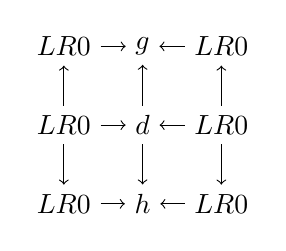
\begin{tikzpicture}
      \node (1t) at (0,2) {$ LR 0 $};
      \node (2t) at (1,2) {$ g $};
      \node (3t) at (2,2) {$ LR 0 $};
      \node (1m) at (0,1) {$ LR 0 $};
      \node (2m) at (1,1) {$ d $};
      \node (3m) at (2,1) {$ LR 0 $};
      \node (1b) at (0,0) {$ LR 0 $};
      \node (2b) at (1,0) {$ h $};
      \node (3b) at (2,0) {$ LR 0 $};
      \draw [->] (1t) to node [] {\scriptsize{$  $}} (2t);
      \draw [->] (3t) to node [] {\scriptsize{$  $}} (2t);
      \draw [->] (1m) to node [] {\scriptsize{$  $}} (2m);
      \draw [->] (3m) to node [] {\scriptsize{$  $}} (2m);
      \draw [->] (1b) to node [] {\scriptsize{$  $}} (2b);
      \draw [->] (3b) to node [] {\scriptsize{$  $}} (2b);
      \draw [->] (1m) to node [] {\scriptsize{$  $}} (1t);
      \draw [->] (1m) to node [] {\scriptsize{$  $}} (1b);
      \draw [->] (2m) to node [] {\scriptsize{$  $}} (2t);
      \draw [->] (2m) to node [] {\scriptsize{$  $}} (2b);
      \draw [->] (3m) to node [] {\scriptsize{$  $}} (3t);
      \draw [->] (3m) to node [] {\scriptsize{$  $}} (3b);
    \end{tikzpicture}
  \]
  % 
  in the double category $ \Lang ( \StrCsp_L , P' ) $.
\end{theorem}

\begin{proof}
  We show sufficiency by induction on the length of the derivation. If
  $ \dderiv{g}{h} $
  %
  \[
  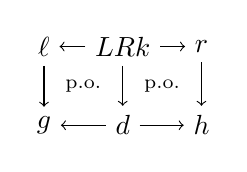
\begin{tikzpicture}
    \node (1t) at (0,1) {$ \ell $};
    \node (2t) at (1,1) {$ LRk $};
    \node (3t) at (2,1) {$ r $};
    \node (1b) at (0,0) {$ g $};
    \node (2b) at (1,0) {$ d $};
    \node (3b) at (2,0) {$ h $};
    \draw [->] (2t) to node [] {\scriptsize{$  $}} (1t);
    \draw [->] (2t) to node [] {\scriptsize{$  $}} (3t);
    \draw [->] (2b) to node [] {\scriptsize{$  $}} (1b);
    \draw [->] (2b) to node [] {\scriptsize{$  $}} (3b);
    \draw [->] (1t) to node [] {\scriptsize{$  $}} (1b);
    \draw [->] (2t) to node [] {\scriptsize{$  $}} (2b);
    \draw [->] (3t) to node [] {\scriptsize{$  $}} (3b);
    \node () at (0.5,0.5) {\scriptsize{p.o.}};
    \node () at (1.5,0.5) {\scriptsize{p.o.}};
  \end{tikzpicture}
  \]
  % 
  the desired square is the horizontal composition of
  %
  \[
    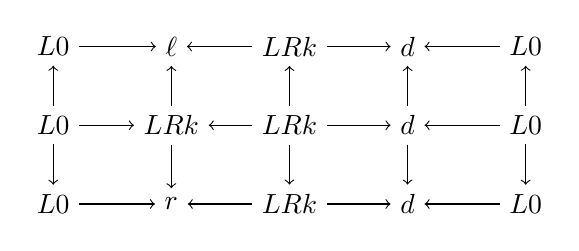
\begin{tikzpicture}
    \begin{scope}
      \node (1t) at (0,2) {$ L0 $};
      \node (2t) at (1.5,2) {$ \ell $};
      \node (3t) at (3,2) {$ LRk $};
      \node (4t) at (4.5,2) {$ d $};
      \node (5t) at (6,2) {$ L0 $};
      \node (1m) at (0,1) {$ L 0 $};
      \node (2m) at (1.5,1) {$ LRk $};
      \node (3m) at (3,1) {$ LRk $};
      \node (4m) at (4.5,1) {$ d $};
      \node (5m) at (6,1) {$ L 0 $};
      \node (1b) at (0,0) {$ L 0 $};
      \node (2b) at (1.5,0) {$ r $};
      \node (3b) at (3,0) {$ LRk $};
      \node (4b) at (4.5,0) {$ d $};
      \node (5b) at (6,0) {$ L 0 $};
      \draw [->] (1t) to node [] {\scriptsize{$  $}} (2t);
      \draw [->] (3t) to node [] {\scriptsize{$  $}} (2t);
      \draw [->] (3t) to node [] {\scriptsize{$  $}} (4t);
      \draw [->] (5t) to node [] {\scriptsize{$  $}} (4t);
      \draw [->] (1m) to node [] {\scriptsize{$  $}} (2m);
      \draw [->] (3m) to node [] {\scriptsize{$  $}} (2m);
      \draw [->] (3m) to node [] {\scriptsize{$  $}} (4m);
      \draw [->] (5m) to node [] {\scriptsize{$  $}} (4m);
      \draw [->] (1b) to node [] {\scriptsize{$  $}} (2b);
      \draw [->] (3b) to node [] {\scriptsize{$  $}} (2b);
      \draw [->] (3b) to node [] {\scriptsize{$  $}} (4b);
      \draw [->] (5b) to node [] {\scriptsize{$  $}} (4b);
      \draw [->] (1m) to node [] {\scriptsize{$  $}} (1t);
      \draw [->] (1m) to node [] {\scriptsize{$  $}} (1b);
      \draw [->] (2m) to node [] {\scriptsize{$  $}} (2t);
      \draw [->] (2m) to node [] {\scriptsize{$  $}} (2b);
      \draw [->] (3m) to node [] {\scriptsize{$  $}} (3t);
      \draw [->] (3m) to node [] {\scriptsize{$  $}} (3b);
      \draw [->] (4m) to node [] {\scriptsize{$  $}} (4t);
      \draw [->] (4m) to node [] {\scriptsize{$  $}} (4b);
      \draw [->] (5m) to node [] {\scriptsize{$  $}} (5t);
      \draw [->] (5m) to node [] {\scriptsize{$  $}} (5b);
    \end{scope}
    \end{tikzpicture}
  \]
  %
  The left square is a generator and the right square is the
  identity on the horizontal arrow $ LRk + L \empty \to d $. The
  square for a derivation $ \dderiv{\deriv{g}{h}}{j} $ is the vertical
  composition of
  %
  \[
    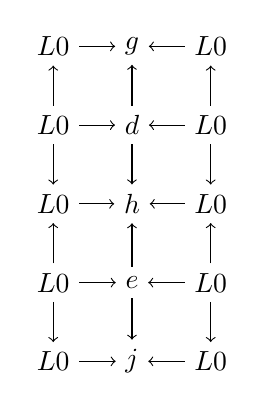
\begin{tikzpicture}
      \node (1t) at (0,4) {$ L 0 $};
      \node (2t) at (1,4) {$ g $};
      \node (3t) at (2,4) {$ L 0 $};
      \node (1m) at (0,3) {$ L 0 $};
      \node (2m) at (1,3) {$ d $};
      \node (3m) at (2,3) {$ L 0 $};
      \node (1b) at (0,2) {$ L 0 $};
      \node (2b) at (1,2) {$ h $};
      \node (3b) at (2,2) {$ L 0 $};
      \node (1bb) at (0,1) {$ L 0 $};
      \node (2bb) at (1,1) {$ e $};
      \node (3bb) at (2,1) {$ L 0 $};
      \node (1bbb) at (0,0) {$ L 0 $};
      \node (2bbb) at (1,0) {$ j $};
      \node (3bbb) at (2,0) {$ L 0 $};
      \draw [->] (1t) to node [] {\scriptsize{$  $}} (2t);
      \draw [->] (3t) to node [] {\scriptsize{$  $}} (2t);
      \draw [->] (1m) to node [] {\scriptsize{$  $}} (2m);
      \draw [->] (3m) to node [] {\scriptsize{$  $}} (2m);
      \draw [->] (1b) to node [] {\scriptsize{$  $}} (2b);
      \draw [->] (3b) to node [] {\scriptsize{$  $}} (2b);
      \draw [->] (1m) to node [] {\scriptsize{$  $}} (1t);
      \draw [->] (1m) to node [] {\scriptsize{$  $}} (1b);
      \draw [->] (2m) to node [] {\scriptsize{$  $}} (2t);
      \draw [->] (2m) to node [] {\scriptsize{$  $}} (2b);
      \draw [->] (3m) to node [] {\scriptsize{$  $}} (3t);
      \draw [->] (3m) to node [] {\scriptsize{$  $}} (3b);
      \draw [->] (1bb) to node [] {\scriptsize{$  $}} (2bb);
      \draw [->] (3bb) to node [] {\scriptsize{$  $}} (2bb);
      \draw [->] (1bbb) to node [] {\scriptsize{$  $}} (2bbb);
      \draw [->] (3bbb) to node [] {\scriptsize{$  $}} (2bbb);
      \draw [->] (1bb) to node [] {\scriptsize{$  $}} (1b);
      \draw [->] (1bb) to node [] {\scriptsize{$  $}} (1bbb);
      \draw [->] (2bb) to node [] {\scriptsize{$  $}} (2b);
      \draw [->] (2bb) to node [] {\scriptsize{$  $}} (2bbb);
      \draw [->] (3bb) to node [] {\scriptsize{$  $}} (3b);
      \draw [->] (3bb) to node [] {\scriptsize{$  $}} (3bbb);
    \end{tikzpicture}
  \]
  %
  The top square is from $ \deriv{g}{h} $ and the second from
  $ \dderiv{h}{j} $.

  Conversely, proceed by structural induction on the generating
  squares of $ \Lang ( \StrCsp_L , P' ) $.  It suffices to show that
  the rewrite relation is preserved by vertical and composition by a
  generating square.  Suppose we have a square
  %
  \[
    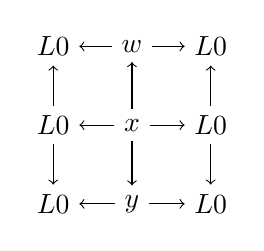
\begin{tikzpicture}
      \node (1t) at (0,2) {$ L 0 $};
      \node (2t) at (1,2) {$ w $};
      \node (3t) at (2,2) {$ L 0 $};
      \node (1m) at (0,1) {$ L 0 $};
      \node (2m) at (1,1) {$ x $};
      \node (3m) at (2,1) {$ L 0 $};
      \node (1b) at (0,0) {$ L 0 $};
      \node (2b) at (1,0) {$ y $};
      \node (3b) at (2,0) {$ L 0 $};
      \draw [->] (2t) to node [] {\scriptsize{$  $}} (1t);
      \draw [->] (2t) to node [] {\scriptsize{$  $}} (3t);
      \draw [->] (2m) to node [] {\scriptsize{$  $}} (1m);
      \draw [->] (2m) to node [] {\scriptsize{$  $}} (3m);
      \draw [->] (2b) to node [] {\scriptsize{$  $}} (1b);
      \draw [->] (2b) to node [] {\scriptsize{$  $}} (3b);
      \draw [->] (1m) to node [] {\scriptsize{$  $}} (1t);
      \draw [->] (2m) to node [] {\scriptsize{$  $}} (2t);
      \draw [->] (3m) to node [] {\scriptsize{$  $}} (3t);
      \draw [->] (1m) to node [] {\scriptsize{$  $}} (1b);
      \draw [->] (2m) to node [] {\scriptsize{$  $}} (2b);
      \draw [->] (3m) to node [] {\scriptsize{$  $}} (3b);
    \end{tikzpicture}
  \]
  % 
  corresponding to a derivation $ \deriv{w}{y} $. Composing this
  vertically with a generating square, which must have form
  %
  \[
    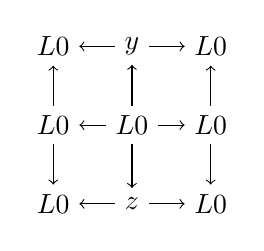
\begin{tikzpicture}
      \node (1t) at (0,2) {$ L 0 $};
      \node (2t) at (1,2) {$ y $};
      \node (3t) at (2,2) {$ L 0 $};
      \node (1m) at (0,1) {$ L 0 $};
      \node (2m) at (1,1) {$ L 0 $};
      \node (3m) at (2,1) {$ L 0 $};
      \node (1b) at (0,0) {$ L 0 $};
      \node (2b) at (1,0) {$ z $};
      \node (3b) at (2,0) {$ L 0 $};
      \draw [->] (2t) to node [] {\scriptsize{$  $}} (1t);
      \draw [->] (2t) to node [] {\scriptsize{$  $}} (3t);
      \draw [->] (2m) to node [] {\scriptsize{$  $}} (1m);
      \draw [->] (2m) to node [] {\scriptsize{$  $}} (3m);
      \draw [->] (2b) to node [] {\scriptsize{$  $}} (1b);
      \draw [->] (2b) to node [] {\scriptsize{$  $}} (3b);
      \draw [->] (1m) to node [] {\scriptsize{$  $}} (1t);
      \draw [->] (2m) to node [] {\scriptsize{$  $}} (2t);
      \draw [->] (3m) to node [] {\scriptsize{$  $}} (3t);
      \draw [->] (1m) to node [] {\scriptsize{$  $}} (1b);
      \draw [->] (2m) to node [] {\scriptsize{$  $}} (2b);
      \draw [->] (3m) to node [] {\scriptsize{$  $}} (3b);
    \end{tikzpicture}
  \]
  %
  corresponding to a production $ 0 \to y + z $ gives
  %
  \[
    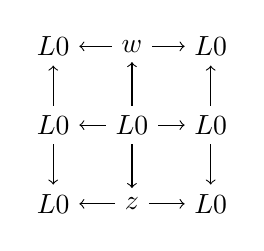
\begin{tikzpicture}
      \node (1t) at (0,2) {$ L 0 $};
      \node (2t) at (1,2) {$ w $};
      \node (3t) at (2,2) {$ L 0 $};
      \node (1m) at (0,1) {$ L 0 $};
      \node (2m) at (1,1) {$ L 0 $};
      \node (3m) at (2,1) {$ L 0 $};
      \node (1b) at (0,0) {$ L 0 $};
      \node (2b) at (1,0) {$ z $};
      \node (3b) at (2,0) {$ L 0 $};
      \draw [->] (2t) to node [] {\scriptsize{$  $}} (1t);
      \draw [->] (2t) to node [] {\scriptsize{$  $}} (3t);
      \draw [->] (2m) to node [] {\scriptsize{$  $}} (1m);
      \draw [->] (2m) to node [] {\scriptsize{$  $}} (3m);
      \draw [->] (2b) to node [] {\scriptsize{$  $}} (1b);
      \draw [->] (2b) to node [] {\scriptsize{$  $}} (3b);
      \draw [->] (1m) to node [] {\scriptsize{$  $}} (1t);
      \draw [->] (2m) to node [] {\scriptsize{$  $}} (2t);
      \draw [->] (3m) to node [] {\scriptsize{$  $}} (3t);
      \draw [->] (1m) to node [] {\scriptsize{$  $}} (1b);
      \draw [->] (2m) to node [] {\scriptsize{$  $}} (2b);
      \draw [->] (3m) to node [] {\scriptsize{$  $}} (3b);
    \end{tikzpicture}
  \]
  %
  which corresponds to a derivation $ \dderiv{\deriv{w}{y}}{z} $.
  Composing horizontally with a generating square
  %
  \[
    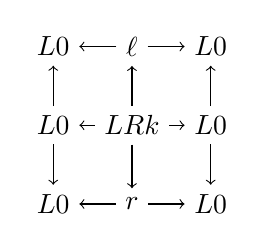
\begin{tikzpicture}
      \node (1t) at (0,2) {$ L 0 $};
      \node (2t) at (1,2) {$ \ell $};
      \node (3t) at (2,2) {$ L 0 $};
      \node (1m) at (0,1) {$ L 0 $};
      \node (2m) at (1,1) {$ LRk $};
      \node (3m) at (2,1) {$ L 0 $};
      \node (1b) at (0,0) {$ L 0 $};
      \node (2b) at (1,0) {$ r $};
      \node (3b) at (2,0) {$ L 0 $};
      \draw [->] (2t) to node [] {\scriptsize{$  $}} (1t);
      \draw [->] (2t) to node [] {\scriptsize{$  $}} (3t);
      \draw [->] (2m) to node [] {\scriptsize{$  $}} (1m);
      \draw [->] (2m) to node [] {\scriptsize{$  $}} (3m);
      \draw [->] (2b) to node [] {\scriptsize{$  $}} (1b);
      \draw [->] (2b) to node [] {\scriptsize{$  $}} (3b);
      \draw [->] (1m) to node [] {\scriptsize{$  $}} (1t);
      \draw [->] (2m) to node [] {\scriptsize{$  $}} (2t);
      \draw [->] (3m) to node [] {\scriptsize{$  $}} (3t);
      \draw [->] (1m) to node [] {\scriptsize{$  $}} (1b);
      \draw [->] (2m) to node [] {\scriptsize{$  $}} (2b);
      \draw [->] (3m) to node [] {\scriptsize{$  $}} (3b);
    \end{tikzpicture}
  \]
  %
  corresponding with a production $ LRk \to \ell + r $ results in the
  square
  %
  \[
    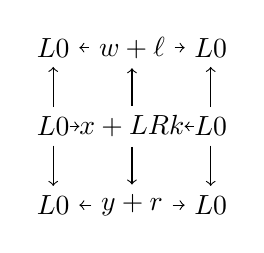
\begin{tikzpicture}
      \node (1t) at (0,2) {$ L 0 $};
      \node (2t) at (1,2) {$ w + \ell $};
      \node (3t) at (2,2) {$ L 0 $};
      \node (1m) at (0,1) {$ L 0 $};
      \node (2m) at (1,1) {$ x + LRk $};
      \node (3m) at (2,1) {$ L 0 $};
      \node (1b) at (0,0) {$ L 0 $};
      \node (2b) at (1,0) {$ y + r $};
      \node (3b) at (2,0) {$ L 0 $};
      \draw [->] (2t) to node [] {\scriptsize{$  $}} (1t);
      \draw [->] (2t) to node [] {\scriptsize{$  $}} (3t);
      \draw [->] (2m) to node [] {\scriptsize{$  $}} (1m);
      \draw [->] (2m) to node [] {\scriptsize{$  $}} (3m);
      \draw [->] (2b) to node [] {\scriptsize{$  $}} (1b);
      \draw [->] (2b) to node [] {\scriptsize{$  $}} (3b);
      \draw [->] (1m) to node [] {\scriptsize{$  $}} (1t);
      \draw [->] (2m) to node [] {\scriptsize{$  $}} (2t);
      \draw [->] (3m) to node [] {\scriptsize{$  $}} (3t);
      \draw [->] (1m) to node [] {\scriptsize{$  $}} (1b);
      \draw [->] (2m) to node [] {\scriptsize{$  $}} (2b);
      \draw [->] (3m) to node [] {\scriptsize{$  $}} (3b);
    \end{tikzpicture}
  \]
  %
  But $ \deriv{w+\ell}{y+r} $ as seen in Lemma
  \ref{thm:rewrite-rel-is-additive}. 

\end{proof}

With this result, we have completely described the rewrite relation
for a grammar $ ( \X , P ) $ with those squares in
$ \Lang ( \StrCsp_L , P' ) $ framed by the initial object of $ \X $.
These squares are rewrites of a closed system, which may be difficult
to understand.  We can instead begin with a closed system as
represented by a horizontal arrow in $ \Lang ( \StrCsp_L , P' ) $ and
decompose it into a composite of easier to understand sub-systems,
rather a sequence of composable horizontal arrows. Rewriting can be
performed on each of these sub-systems which, of course, is
represented by squares. The composite of these squares gives are
rewriting of the original system.  






% ~~~~~~~~~~~~~~~~~~~~~~~~~~~~~~~~~~~~~~~~
% 
% ~~~~~~~~~~~ bibliography ~~~~~~~~~~~~~~~
% 
% ~~~~~~~~~~~~~~~~~~~~~~~~~~~~~~~~~~~~~~~~

\begin{thebibliography}{99}
  % use APA style
  % \bibitem{1st-citation}

\bibitem{StrCsp} J.~Baez, K.~Courser. Structured cospans. \emph{In preparation}.

\bibitem{NetMods} J.~Baez, J.~Foley, J.~Moeller, B.~Pollard. Network
  Models. \emph{arXiv preprint} arXiv:1711.00037. 2017.
  
\bibitem{PassiveNets} J.~Baez, B.~Fong. A compositional framework for passive linear networks. \emph{arXiv preprint} arXiv:1504.05625. 2015.

\bibitem{MrkvProc} J.~Baez, B.~Fong, B.~Pollard. A compositional
  framework for Markov processes. \emph{J.~Math.~Phys.} 57, No.~3:
  033301. 2016.
  
\bibitem{RxNets} J.~Baez, B.~Pollard. A compositional framework for
  reaction networks. \emph{Rev. Math. Phys.} 29, No.~9, 1750028. 2017.

\bibitem{OpenPetri} J.~Baez, J.~Master. Open Petri Nets. \emph{arXiv preprint} arXiv:1808.05415. 2018.
  
\bibitem{Chomsky} N.~Chomsky. On Certain Formal Properties of Grammars.
\emph{Inf.~Control}. No.~2. 137-167. 1959. 
  
\bibitem{Cic_SpCsp} D.\ Cicala. Spans of cospans. \emph{Theory Appl.\
    Categ.} 33, No.\ 6, 131--147. 2018.

\bibitem{CicCour_SpCspTopos} D.\ Cicala and K.\ Courser. Spans of
  cospans in a topos. \emph{Theory Appl.\ Categ.} 33, No.\ 1,
  1--22. 2018.

\bibitem{DixKiss_OpenGraphs} L.\ Dixon, and A.\ Kissinger. Open-graphs
  and monoidal theories. \emph{Math.\ Structures Comput.\ Sci.},
  \textbf{23}, No.\ 2, 308--359. 2013.

\bibitem{Ehrig_GraphGram} H.\ Ehrig, M.\ Pfender, and H.J.\
  Schneider. Graph-grammars: An algebraic approach. In \emph{Switching
    and Automata Theory, 1973. SWAT'08. IEEE Conference Record of 14th
    Annual Symposium on}, 167--180. IEEE. 1973.
  
\bibitem{DecorCsp} B.\ Fong. Decorated cospans. \emph{Theory
    Appl.\ Categ.} 30, Paper No.\ 33, 1096--1120. 2015.
          
\bibitem{Gadd_IndGraphTrans} F.\ Gadducci, R.\ Heckel. An inductive
  view of graph transformation.\emph{International Workshop on
    Algebraic Development Techniques}. 223--237. Springer, Berlin. 1998.

\bibitem{DblPushoutRevis} A.~Habel, J.~M\:{u}ller,
  D.~Plump. Double-pushout graph transformation
  revisited. \emph{Math. Structures Comput. Sci.}
  11. No.~5. 637--688. 2001).
  
\bibitem{LackSobo_Adhesive} S.\ Lack, and P.\ Soboci\'{n}ski. Adhesive
  categories. In \emph{International Conference on Foundations of
    Software Science and Computation Structures}, 273--288. Springer,
  Berlin, Heidelberg. 2004.

\bibitem{LackSobo_ToposIsAdh} S.~Lack, P.~Soboci\'{n}ski. Toposes are adhesive. \emph{International Conference on Graph Transformation}. Springer, Berlin, Heidelberg. 2006.

\bibitem{ShulDblCat} M.~Shulman. Constructing symmetric monoidal bicategories. \emph{arXiv preprint} arXiv:1004.0993. 2010.
  
\bibitem{Wraith_ArtinGlue} G.\ Wraith. Artin gluing. \emph{J.\ Pure
    Appl.\ Algebra} \textbf{4}, 345--348. 1974.

\end{thebibliography}

\end{document}
